\documentclass[11pt]{article}
\usepackage[a4paper,margin=25mm]{geometry}
\usepackage{amsmath,amssymb,amsthm}
\numberwithin{equation}{section}
\usepackage{graphicx,booktabs,tabularx,siunitx,placeins}
\renewcommand{\tabularxcolumn}[1]{>{\raggedright\arraybackslash}p{#1}}
\usepackage[font=small,labelfont=bf]{caption}
\usepackage[numbers,sort&compress]{natbib}
\usepackage{xurl}
\usepackage[hidelinks]{hyperref}
\setlength{\emergencystretch}{2em}
\setlength{\tabcolsep}{5pt}
\renewcommand{\arraystretch}{1.15}
\setcounter{topnumber}{3}
\renewcommand{\topfraction}{.85}
\renewcommand{\textfraction}{.10}
\renewcommand{\floatpagefraction}{.70}
\raggedbottom
\bibliographystyle{unsrtnat}

\title{Random Feature Galerkin Methods for Accuracy-Matched Incompressible Flow:\\Discretization, GPU Kernels, and End-to-End Performance Attribution}
\author{Xingchen Liu\\School of Mathematics, Sichuan University}
\date{}
\hypersetup{pdftitle={Random Feature Galerkin Methods for Accuracy-Matched Incompressible Flow: Discretization, GPU Kernels, and End-to-End Performance Attribution},pdflang={en}}
\begin{document}
\maketitle
\begin{abstract}
We study numerical adaptations and low-level implementations of a fixed random feature Galerkin solver for incompressible flow, separating the effects of the trial space, time schedule, operator cost, and runtime overhead. For two-dimensional flow in a finite annulus without imposed reflection symmetry, we specify boundary-compatible features, weighted rank truncation, and a weak discretization with an independent mean-flow block. We derive a variable-step SBDF2 bridge with boundary lifting and establish its local consistency. Common coordinates for the time-phase matrices of each angular mode yield a geometric anchor that minimizes a stated worst-case condition-number bound. The implementation analysis describes FP64 FFT packing and shared-memory fusion, warp-level probe reduction, native C radial kernels, and setup and compilation-artifact reuse. At $Re=100$ and $T=72$, all 78 GPU trajectories, comprising 39 configurations under two cache policies, meet the prescribed $0.5\%$ velocity and vorticity tolerances. Piecewise schedules remove $11.11\%$ and $9.36\%$ of true nonlinear evaluations. FFT fusion reduces short-trajectory marching time by $9\%$--$17\%$ but increases the first full-solve cost by $23\%$--$69\%$. Twenty new CPU trajectories supplement feature and switch controls. Both fixed-midpoint frequency configurations qualify with analytic layers, while all 12 configurations without nonzero-mode layers fail; retained rank also decreases, so this is not an equal-rank enrichment ablation. Delaying the switch only modestly improves accuracy at greater nonlinear cost, and radial/modal profiles distinguish the distribution of velocity and vorticity errors. Reduced Legendre spaces also qualify, and the final isolated timing campaign is not accepted; an overall speed advantage over comparably optimized traditional CFD therefore remains unestablished. The contribution is a reproducible combination of discrete derivations, source-level cost explanations, and scoped positive and negative evidence. Local consistency, transformed conditioning, and numerical qualification are not interpreted as guarantees of nonlinear stability or universal performance.

\par\smallskip
\noindent\textbf{Keywords}\quad Random features, incompressible Navier--Stokes equations, Galerkin methods, variable-step SBDF2, GPU kernels, performance attribution
\end{abstract}
\section{Introduction}
\label{sec:introduction}

Neural features provide alternatives to polynomial trial spaces for partial differential equations. A flow solver, however, combines a representation, spatial projection, time integration, linear algebra, nonlinear transforms, and runtime management. A speedup observed after changing several of these components cannot be attributed automatically to random features. This study examines that attribution problem for a fixed random feature Galerkin discretization of two-dimensional unsteady incompressible flow, and asks how its mathematical structure translates into measurable computational savings.

Unsteady wakes make the comparison demanding. Velocity involves first derivatives of the streamfunction, whereas vorticity involves second derivatives; a small velocity error can therefore coexist with a substantially larger vorticity error. Alternating shedding also accumulates phase error. Independently shifting each trajectory in time can make plots agree without recovering the original initial-boundary-value solution. Meanwhile, a small GPU operator may take only tens of microseconds, even when compilation, module loading, FFT planning, and context initialization consume a substantial fraction of the full solve. We consequently require common physical accuracy, original time coordinates, and explicit end-to-end cost boundaries.

The test problem is a finite annulus at $Re=100$, integrated to $T=72$ without imposed reflection symmetry. The radial approximations use fixed random trigonometric features, deterministic Legendre features, or fourth-order spatial finite differences. All retain the full real Fourier representation in angle and solve the same physical problem with second-order time integration. Legendre--Galerkin is itself a traditional CFD baseline and must be included in that category. The fixed-feature solver is distinct from a PINN that trains a representation of an entire trajectory by residual minimization.

Three questions organize the study. First, how much actual work can piecewise time steps and smaller retained spaces remove while preserving both velocity and vorticity accuracy? Second, which costs do common phase coordinates, FFT fusion, and parallel observation change, and can other implementation costs offset the algebraic savings? Third, does the available evidence establish an overall advantage over strong deterministic baselines under matched accuracy, initialization policies, and timing boundaries? These questions require discrete analysis, operator experiments, and complete isolated runs, respectively; one local speedup cannot answer all three.

\begin{table}[!htbp]
\centering\small
\caption{Classification of the work and its evidential limits. A numerical adaptation is distinct from a new basic algorithm; a local speedup is distinct from a full-solve advantage.}
\label{tab:contribution-map}
\begin{tabularx}{\linewidth}{@{}>{\raggedright\arraybackslash}p{.20\linewidth}XXX@{}}
\toprule
Component & Category & Available evidence & Limit \\
\midrule
Lifting and one variable-step bridge & Numerical-method adaptation & Consistency derivation and trajectory qualification & No unconditional stability theorem for the full NS system \\
Common phase coordinates and anchor & Linear algebra analysis & Same-mode identities and a spectral bound & Bound minimization does not minimize measured runtime \\
Retained radial spaces and Legendre control & Discretization and validation & Five fixed seeds and reduced deterministic spaces & No universal random-feature advantage \\
Fused FFT, warp observations, C kernels & Low-level implementation & Source, local tests, short trajectories & Application kernels, not a third-party FFT library patch \\
Shared setup, caching, startup path & Runtime engineering & Stage records and cache equivalence & Final isolated ranking remains unestablished \\
\bottomrule
\end{tabularx}
\end{table}

The principal results are verifiable workload reductions and performance attribution. The two time schedules remove approximately $11.11\%$ and $9.36\%$ of true nonlinear evaluations. All 78 GPU trajectories, covering 39 configurations under two cache policies, satisfy the registered numerical criteria. The specialized fused FFT is effective on fixed states and during short trajectory advancement, yet increases the cost of the first complete solve. The final isolated timing campaign failed its acceptance criteria, and its remaining records are not used to rank methods. These limits position the paper as numerical computation and application-level high-performance computing research. The evidence does not establish a general convergence theory or a universal speed advantage over traditional CFD.

Additional factorial ablations examine whether randomness is necessary: both fixed-midpoint frequency configurations qualify when analytic layers are retained, while all 12 configurations without nonzero-mode layers fail the field criterion and also lose retained rank. The conclusion is therefore restricted to the effectiveness of the present enriched spaces, without automatically attributing it to random sampling. Section~\ref{sec:review-experiments} adds radial/modal error decomposition and delayed-switch controls; Section~\ref{sec:geometry-scope} identifies the algebraic structure lost on nonseparable geometries.

\section{Related work and scope}
\label{sec:related-work}

\subsection{Random features, projection solvers, and trained representations}

The random feature method fixes nonlinear features and determines their combination coefficients for PDE approximation\cite{r1}. Local extreme learning machines combine fixed hidden layers with domain decomposition\cite{r2}; randomized neural network Petrov--Galerkin methods have been applied to elasticity and Navier--Stokes equations\cite{r3}. High-precision RFM, randomized preconditioning, and orthogonal feature learning address accuracy, conditioning, and representation quality\cite{r4,r5,r6}. Random features combined with Galerkin projection, preconditioning, or orthogonalization are consequently not standalone novelty claims of this work.

Time-dependent RFM can also use space-time features and partitions of unity, with global or blockwise least-squares solves\cite{r15}. The present implementation takes a different route: random features define only the radial trial space, Fourier modes represent angle, and a stepwise IMEX scheme advances time. It neither learns temporal features nor repeatedly minimizes a trajectory-wide residual. Error statements for block propagation in space-time least squares therefore require a separate derivation before being applied to this SBDF2 evolution, and performance results do not transfer automatically between the formulations.

PINNs use automatic differentiation to construct residual losses and train network parameters\cite{r7}. Causal training changes the treatment of temporal learning, while PirateNets use adaptive residual connections to improve deep PINN optimization\cite{r8,r16}. A comparison with such methods must account for training, restarts, sampling, inference, and derivative reconstruction according to the intended use. Published errors and times from different geometries, boundaries, horizons, or hardware cannot be inserted into an accuracy-matched table here. No complete trained-model comparison on this same problem and tolerance is available in the present evidence. These references delimit the scope rather than establish a speed ranking.

\subsection{Time discretization and linear algebra}

IMEX multistep methods and variable-step extensions are established approaches\cite{r9,r12}. The second-order coefficients used here belong to that framework. Our analysis concerns their compatibility with the discrete mass, boundary lifting, contracted flux histories, and a single step-size transition in this implementation. Likewise, whitening and diagonalizing a symmetric definite generalized eigenproblem use standard linear algebra\cite{r10}. The relevant questions are whether multiple time phases of one angular mode can share coordinates, what an anchor selection actually optimizes, and why fewer factorizations can still increase setup cost when the original device interface is retained.

\subsection{GPU fusion and application performance}

FFT dealiasing, Hermitian representations of real fields, and mixed-radix transforms are established techniques\cite{r11,r13}. cuFFTDx already provides device FFTs, fused convolution examples, and comparisons with cuFFT\cite{r17}; warp exchange and reduction use standard CUDA programming mechanisms\cite{r18}. The engineering work here implements and checks these mechanisms for a particular FP64 multifield flux layout, including channel-scale sensitivity, startup overhead, and unsuccessful candidates. It does not introduce the general idea of FFT fusion as a new FFT algorithm.

High-level languages can organize high-performance flow solvers whose computational kernels execute in compiled libraries or native implementations\cite{r14}. We therefore discuss bottlenecks through data movement, synchronization, matrix layout, and lifecycle cost. Choosing C, CUDA, or another host language should follow the measured cost fraction and the work that can actually be removed. The same reasoning applies to an upstream contribution: the present changes are application-side kernels, with no modification of third-party library source. A reusable upstream sample needs independent correctness, an equivalent library-based comparison, and a reproducible build; a local application speedup alone does not constitute a library performance fix.

\section{Flow model and the fixed approximation space}
\label{sec:governing-equations}
\label{sec:space-discretization}

\subsection{A driven finite-annulus problem}

We consider the two-dimensional incompressible Navier--Stokes equations
\begin{equation}
 \partial_t\boldsymbol u+(\boldsymbol u\cdot\nabla)\boldsymbol u
 =-\nabla p+\nu\Delta\boldsymbol u,\qquad
 \nabla\cdot\boldsymbol u=0,\qquad
 \Omega=\{(r,\theta):a<r<R\}.
 \label{eq:ns}
\end{equation}
The cylinder diameter and the final streamwise speed define the length
and velocity scales. The calculations use \(a=0.5\), \(R=6\),
\(\nu=0.01\), and hence \(\mathrm{Re}=100\). The final time is
\(T=72\). Introduce the logarithmic radial coordinate
\(s=\log(r/a)\), its extent \(L=\log(R/a)\), and \(z=s/L\).
The area measure becomes \(r^2\,ds\,d\theta\). The physical radial span is $R-a=5.5$; it is not the logarithmic extent $L=\log12$ used in the formulas.

For nonzero angular modes, a streamfunction gives
\begin{equation}
 u_r=\frac{\psi_\theta}{r},\qquad
 u_\theta=-\frac{\psi_s}{r},\qquad
 \omega=-\frac{\psi_{ss}+\psi_{\theta\theta}}{r^2}.
 \label{eq:kinematics}
\end{equation}
The azimuthal mean is advanced separately as a real tangential velocity
\(v(s,t)\); its radial velocity is zero and its vorticity is
\((v+v_s)/r\). This representation preserves all sine and cosine
components of every retained nonzero mode and does not impose a
reflection or zero-circulation constraint. The pressure is eliminated
from the nonzero-mode equations by taking the curl; the mean tangential
momentum equation supplies the remaining velocity block.

The initially stationary flow is driven by
\begin{equation}
 U(t)=1-e^{-(t/0.8)^3},\qquad
 V(t)=\begin{cases}
 0.12\sin^4[\pi(t-4)/8],&4<t<12,\\
 0,&\text{otherwise}.
 \end{cases}
 \label{eq:driving}
\end{equation}
The finite-duration transverse pulse breaks reflection symmetry. At
the inner boundary, \(\psi=\psi_s=0\). At the outer boundary, the
nonzero modes satisfy
\begin{equation}
 \psi(L,\theta,t)=R[U(t)\sin\theta-V(t)\cos\theta],\qquad
 \omega(L,\theta,t)=0.
 \label{eq:outer-boundary}
\end{equation}
The separate mean block satisfies \(v(0,t)=0\) and
\(v_s(L,t)+v(L,t)=0\). Thus the outer circle does not have a full
velocity Dirichlet condition. It is part of the definition of the
finite-domain problem, rather than an exact transparent boundary for
unbounded cylinder flow.

The prescribed boundary data are represented by a lifting
\begin{equation}
 \begin{gathered}
 \psi_\ell(s,\theta,t)=\ell(s)[U(t)\sin\theta-V(t)\cos\theta],\\
 \ell(s)=R[(1-\beta)z^2+\beta z^3],\quad
 \beta=\frac{L^2-2}{4}.
 \end{gathered}
 \label{eq:lifting}
\end{equation}
It obeys \(\ell(0)=\ell_s(0)=0\), \(\ell(L)=R\), and
\(\ell_{ss}(L)=R\). The last identity enforces zero outer vorticity
for the lifted \(k=1\) mode. With the convention
\(f=c_0+2\operatorname{Re}\sum_{k=1}^{K}c_ke^{ik\theta}\),
the complex lifting amplitude is \(g(t)=-(V(t)+iU(t))/2\).
The same convention is used in reconstruction, nonlinear projection,
and error scoring; conjugate negative modes represent the complete
real field.

The finite outer radius is a material limitation. In the archived
domain-size diagnostic, increasing \(R\) from 6 to 8 changed the
unaligned vorticity by about \(50.39\%\) in the common \(r\leq4\)
region, and also changed the shedding frequency. The numerical
tolerance below is therefore a tolerance for the specified
\(R=6\) problem. Domain truncation and discretization error are not
interchangeable.

\subsection{Random and deterministic radial trial functions}

Write the nonzero streamfunction coefficients as
\begin{equation}
 \psi_k(s,t)=\sum_{j=1}^{d}F_j(s)x_{jk}(t)
                +\delta_{k1}g(t)\ell(s),\qquad 1\leq k\leq K.
 \label{eq:trial-expansion}
\end{equation}
The functions \(F_j\) are fixed before time integration. No neural
network weights are trained along the trajectory. The RFM designation
refers to the randomly chosen radial feature space, followed by a
deterministic Galerkin evolution of its coefficients \cite{r1,r2,r3}.

For an odd input size \(m=2p+1\), the raw random features are a constant
and \(p\) sine--cosine pairs. Specifically,
\begin{equation}
 \begin{gathered}
 b_j=\frac{62}{p}(j+\xi_j),\qquad
 \xi_j\sim\operatorname{Uniform}(0.2,0.8),\\
 q_{j,0}(z)=\cos[b_j(z-\tfrac12)],\quad
 q_{j,1}(z)=\sin[b_j(z-\tfrac12)].
 \end{gathered}
 \label{eq:random-features}
\end{equation}
where \(j=0,\ldots,p-1\). The random draws use a fixed
\texttt{NumPy default\_rng(seed)}. The registered seed set is
\(7331,7687,8011,8353,9041\). The Legendre comparison replaces these
raw functions by \(P_j(2z-1)\), \(j=0,\ldots,m-1\), while retaining
the same boundary transformation, enrichment, quadrature, and time
discretization. The reported cases use no radial coordinate warping.

Boundary conditions are imposed analytically. For a raw function
\(q\), let \(\chi(z)=16z^2(1-z)\) and
\(b(z)=z^2(1-z)^2/2\), and define
\begin{equation}
 \mathcal Bq(z)=\chi(z)q(z)
       -b(z)\left.\frac{d^2(\chi q)}{dz^2}\right|_{z=1}.
 \label{eq:boundary-transform}
\end{equation}
Because \(b(0)=b'(0)=b(1)=0\) and \(b''(1)=1\), this function
satisfies \(F(0)=F_s(0)=F(L)=F_{ss}(L)=0\). Consequently the
homogeneous nonzero modes satisfy both no slip at the cylinder and
zero outer vorticity for every \(k\). Derivatives with respect to
\(s\) include the factors \(L^{-1}\) and \(L^{-2}\); the
correction in \eqref{eq:boundary-transform} is expressed in \(z\).

Both trial families receive the same six analytic outer-layer
functions. For \(\delta=L-s\), these are
\begin{equation}
 E_\gamma(s)=z^2\left[\delta+
       \left(\gamma+\frac{2}{L}\right)\delta^2\right]
       e^{-\gamma\delta},\qquad
 \gamma\in\{16,36,80,165,340,660\}.
 \label{eq:layer-features}
\end{equation}
Their constant and quadratic Taylor coefficients at \(\delta=0\)
vanish, giving the same outer homogeneous conditions; the factor
\(z^2\) supplies the inner conditions. These functions resolve the
outer-boundary layers of this finite-domain formulation. They are not
a learned consequence of the random features.

The mean block uses a deterministic polynomial space in both families.
Its raw functions are
\(z[(L+2)-(L+1)z]\) and
\(z(1-z)^2P_j(2z-1)\), \(j=0,\ldots,m_0-2\), with \(m_0=24\).
The mean enrichment is
\(z[1+(\gamma+1+1/L)\delta]e^{-\gamma\delta}\).
All satisfy the mean boundary conditions. The six enrichments give
30 retained mean functions in the final configurations. Randomness is
therefore restricted to the nonzero-mode radial trial space.

\subsection{Quadrature, rank selection, and the meaning of model size}

Radial integration uses positive composite Gauss weights on
\([0,L-0.12]\), \([L-0.12,L-0.018]\), and \([L-0.018,L]\).
With \(q\) nodes and \(b_q=\max(8,\lfloor q/6\rfloor)\), the
three allocations are \(q-2b_q,b_q,b_q\). For the two principal
Galerkin configurations, these are \(44/11/11\) and \(52/12/12\).
The random trigonometric and exponential radial functions are not
polynomials, so this quadrature is an approximation to the continuous
weak form. Positivity statements below apply exactly to the
quadrature-defined matrices; they are not quadrature-error estimates.

Let \(\widetilde F,\widetilde D,\widetilde D_2\) be the values and
first two \(s\)-derivatives of all raw, boundary-corrected and enriched
functions at the radial nodes. With \(W=\operatorname{diag}(w_i)\),
form
\begin{equation}
 \mathcal A=\operatorname{diag}(\sqrt{w_i}/r_i)
              (\widetilde D_2-\widetilde F),\quad
 S=\operatorname{diag}(\|\mathcal A_{:j}\|_2),\quad
 \mathcal A S^{-1}=U\Sigma V^{\mathsf T}.
 \label{eq:feature-svd}
\end{equation}
All retained raw columns must have nonzero norms. Keep singular values
\(\sigma_j>10^{-10}\sigma_1\), and set
\begin{equation}
 C=S^{-1}V_d\Sigma_d^{-1},\qquad
 F=\widetilde F C,\quad D=\widetilde D C,\quad
 D_2=\widetilde D_2 C.
 \label{eq:feature-transform}
\end{equation}
This is a discrete differential normalization with rank truncation,
rather than an orthogonalization in the ordinary point-value norm.
In exact arithmetic,
\(\operatorname{diag}(\sqrt{w_i}/r_i)(D_2-F)=U_d\).
It therefore normalizes the \(k=1\) dissipation Gram matrix to
\(\nu I\). This identity describes the existing construction; it is
not a newly measured optimization or a guarantee for all angular modes.
The mean block analogously normalizes
\(\operatorname{diag}(\sqrt{w_i})(\widetilde V+\widetilde V_s)\).

An input label such as RFM37 counts raw random features, not unknowns.
Enrichment adds columns and truncation can remove them. The actual
nonzero-mode rank is \(d\), and the real coefficient count is
\(2Kd+d_0\), where \(d_0=30\) is the mean rank. Fixed-rank contrasts
and accuracy-matched contrasts answer different questions. In
particular, a lower RFM input count is not evidence of a lower rank
than a Legendre control. The seed and cutoff are part of the model
identity and must remain fixed when comparing implementations.

\section{Weak formulation and time-discrete algorithms}
\label{sec:numerical-method}

\subsection{Nonzero-mode mass, dissipation, and nonlinear flux}

For the velocity field defined above, incompressibility gives the
vorticity equation in conservative logarithmic coordinates:
\begin{equation}
 r^2\partial_t\omega
  +\partial_s(r u_r\omega)+\partial_\theta(r u_\theta\omega)
   =\nu(\omega_{ss}+\omega_{\theta\theta}).
 \label{eq:vorticity-conservative}
\end{equation}
Test its \(k\)-th Fourier coefficient with a homogeneous radial basis
function. One integration by parts in the mass term after inserting
\(r^2\omega_k=-(\psi_{k,ss}-k^2\psi_k)\) yields the bilinear form
\(\int(F_i'\psi_k'+k^2F_i\psi_k)\,ds\). Integrating the viscous
term twice gives a negative Gram form. The boundary terms vanish
because \(F_i=0\) at both ends, \(F_i'(0)=0\), and
\(\omega_k(L)=0\). Applying the prescribed radial quadrature gives
\begin{align}
 M_k&=D^{\mathsf T}WD+k^2F^{\mathsf T}WF,
       \label{eq:mass}\\
 K_k&=\nu(D_2-k^2F)^{\mathsf T}
        \operatorname{diag}(w_i/r_i^2)(D_2-k^2F).
       \label{eq:dissipation}
\end{align}
For every real coefficient vector \(x\),
\begin{equation}
 \begin{aligned}
 x^{\mathsf T}M_kx&=\|W^{1/2}Dx\|_2^2+k^2\|W^{1/2}Fx\|_2^2,\\
 x^{\mathsf T}K_kx&=\nu\|
    \operatorname{diag}(\sqrt{w_i}/r_i)(D_2-k^2F)x\|_2^2.
 \end{aligned}
 \label{eq:gram-positivity}
\end{equation}
Both matrices are symmetric positive semidefinite in exact
arithmetic. Positive definiteness of \(M_k\) additionally requires
full column rank of the stacked weighted value and derivative samples
on the retained space. The compact form \eqref{eq:dissipation} is
algebraically equivalent to the expanded expression used by the
archived implementation. Its positivity does not remove finite
precision cancellation, assembly asymmetry, or a poorly conditioned
coordinate map.

Let \(a_k\) and \(b_k\) be the Fourier coefficients of
\(u_r\omega\) and \(u_\theta\omega\) evaluated at the radial
nodes. Integration by parts in the two transport terms gives
\begin{equation}
 f_k=D^{\mathsf T}\operatorname{diag}(w_i r_i)a_k
      -ikF^{\mathsf T}\operatorname{diag}(w_i r_i)b_k.
 \label{eq:weak-flux}
\end{equation}
The products use the complete velocity, including the mean block and
boundary lifting. They are evaluated in physical angle and projected
back to the retained spectrum, coupling the otherwise independent
linear mode blocks. This is the reason that making linear solves
diagonal does not eliminate the nonlinear FFT work.

For \(k=1\), the lifting projections are
\begin{equation}
 \begin{aligned}
 M_\ell&=D^{\mathsf T}W\ell_s+F^{\mathsf T}W\ell,\\
 K_\ell&=\nu(D_2-F)^{\mathsf T}
       \operatorname{diag}(w_i/r_i^2)(\ell_{ss}-\ell).
 \end{aligned}
 \label{eq:lift-projections}
\end{equation}
They vanish from the equations of the other modes. Suppressing the
mode index and allowing zero lifting vectors where appropriate, the
semidiscrete system is
\begin{equation}
 m'(t)+Kx(t)+g(t)K_\ell=f(t),\qquad
 m(t)=Mx(t)+g(t)M_\ell.
 \label{eq:semidiscrete}
\end{equation}
The differentiated quantity is the complete weak mass \(m\). Treating
it as \(Mx\) alone would omit the boundary acceleration. Several
independent liftings can be included by replacing each \(gM_\ell\)
and \(gK_\ell\) by the corresponding sum.

\subsection{Why the mean block is a separate equation}

Angular averaging of tangential momentum gives
\begin{equation}
 \partial_t v=-\langle u_r\omega\rangle_\theta
       +\frac{\nu}{r^2}(v_{ss}-v).
 \label{eq:mean-equation}
\end{equation}
Let \(V\) and \(V_s\) now denote the sampled mean basis and its
derivative, rather than the transverse pulse in
\eqref{eq:driving}. The mean matrices and source are
\begin{equation}
 \begin{aligned}
 M_0&=V^{\mathsf T}\operatorname{diag}(w_i r_i^2)V,\qquad
 K_0=\nu(V+V_s)^{\mathsf T}W(V+V_s),\\
 f_0&=-V^{\mathsf T}\operatorname{diag}(w_i r_i^2)a_0.
 \end{aligned}
 \label{eq:mean-matrices}
\end{equation}
To check the dissipation form, expand
\(\int(V+V_s)(v+v_s)\,ds\): its cross terms combine to
\([Vv]_0^L\), which is exactly the boundary contribution obtained
from \(-\int V(v_{ss}-v)\,ds\) using \(v_s(L)=-v(L)\) and
\(v(0)=0\). There is no direct boundary lifting in this block.
The negative radial-flux sign in \eqref{eq:mean-matrices} follows
from tangential momentum. Setting \(k=0\) in
\eqref{eq:mass}--\eqref{eq:weak-flux} would produce a different
representation and is not the implemented mean equation.

\subsection{Constant-step integration and a single bridge}
\label{sec:time-phase}

The baseline treats diffusion implicitly and the nonlinear weak flux
by two-point extrapolation, using SBDF2 \cite{r9,r12}. After the
implicit Euler start, a constant step \(h\) solves
\begin{equation}
 \begin{aligned}
 (\tfrac32M+hK)x_{n+1}
  ={}&2m_n-\tfrac12m_{n-1}+h(2f_n-f_{n-1})\\
   &-g_{n+1}(\tfrac32M_\ell+hK_\ell).
 \end{aligned}
 \label{eq:uniform-sbdf}
\end{equation}
The initialization uses the stationary initial state and the
prescribed smooth startup. Euler startup does not establish
second-order convergence by itself; its consistency with the
initial-value problem must be considered together with the following
multistep evolution. In the implemented initial state the explicit
nonlinear source is zero.

The optimized schedule uses a constant step \(H\) until \(t_0=8\)
and a larger constant step \(h\) afterward. Only the first update
across this interface has unequal consecutive intervals. Write
\(t_-=t_0-H\), \(t_+=t_0+h\), and \(\rho=h/H>0\). Define
\begin{equation}
 a_0=\frac{1+2\rho}{1+\rho},\qquad b_0=1+\rho,\qquad
 b_1=\frac{\rho^2}{1+\rho}.
 \label{eq:bridge-coefficients}
\end{equation}
The bridge is
\begin{equation}
 \begin{aligned}
 (a_0M+hK)x_+={}&b_0m_0-b_1m_-+
 h[(1+\rho)f_0-\rho f_-]\\
 &-g_+(a_0M_\ell+hK_\ell).
 \end{aligned}
 \label{eq:bridge}
\end{equation}
In this subsection \(m_0\) and \(f_0\) refer to time \(t_0\),
not to the azimuthal mean. Historical masses already contain their
historical lifting values; the future lifting is subtracted once.
At \(\rho=1\), \eqref{eq:bridge} reduces exactly to
\eqref{eq:uniform-sbdf}.

\paragraph{Proposition 1 (local consistency of the lifted bridge).}
Assume \(m\in C^4\) and \(f\in C^3\) along a smooth exact
semidiscrete solution in a neighborhood of the bridge. Assume also
that \(\rho\) lies in a fixed compact subset of \((0,\infty)\).
For \(\delta=\max(H,h)\), the derivative-form residual of
\eqref{eq:bridge} is \(O(\delta^2)\), and its step-scaled
equation residual is \(O(h\delta^2)\).

\paragraph{Proof.}
Differentiate the quadratic interpolant through the three masses at
\(t_+\). Its derivative is
\(Dm_+=(a_0m_+-b_0m_0+b_1m_-)/h\).
The linear extrapolant of the two fluxes has value
\((1+\rho)f_0-\rho f_-\) at the same endpoint. Taylor expansion
about \(t_+\) gives
\begin{align}
 Dm_+-m'(t_+)
   &=-\frac{h(h+H)}{6}m'''(t_+)+O(\delta^3),
      \label{eq:bridge-derivative}\\
 (1+\rho)f_0-\rho f_- - f(t_+)
   &=-\frac{h(h+H)}{2}f''(t_+)+O(\delta^3).
      \label{eq:bridge-extrapolation}
\end{align}
Substitute these in \eqref{eq:semidiscrete}, evaluate diffusion and
lifting at \(t_+\), and collect the two residuals. Substitution of
\(m_+=Mx_++g_+M_\ell\) gives the stated bridge. \hfill\(\square\)

This proposition is local consistency, not unconditional stability
or long-time convergence of the nonlinear Navier--Stokes solution.
Those require additional regularity, startup, perturbation, and
stability estimates. The finite-duration pulse is piecewise smooth;
the displayed Taylor argument is local to the bridge at \(t=8\),
which is away from the pulse endpoints. For the scalar zero equation
\(y'=0\), the bridge differences satisfy
\begin{equation}
 y_+-y_0=\frac{\rho^2}{1+2\rho}(y_0-y_-).
 \label{eq:zero-equation}
\end{equation}
The two registered ratios \(8/7\) and \(19/17\) give
\(64/161\) and \(361/935\); the constant segments have factor
\(1/3\). Thus the homogeneous differences are bounded on this
particular grid. Explicit advection and mode coupling are absent
from this check, so it does not supply a flow stability theorem.

The work reduction follows from the schedule rather than from the
trial family. At \(T=72\), changing the rate from 128 to 112 at
\(t=8\) changes the step count from \(9216\) to \(8192\).
Changing 152 to 136 changes \(10944\) to \(9920\). The initial
nonlinear source is identically zero and the Euler state is constructed
before the repeated updates. Nonlinear kernels evaluate the states
at \(t_1,\ldots,t_{N_{\rm step}-1}\); the terminal state needs no
subsequent evaluation. The respective
recorded evaluation counts are \(9215\to8191\) and
\(10943\to9919\). This count does not predict the complete solve
time, which also includes additional phase preparation and startup.

\subsection{Reuse of fixed spatial preparation}

\paragraph{Proposition 2 (exact-arithmetic reuse).}
Fix the geometry, viscosity, feature family, random seed, enrichments,
quadrature, lifting, column scaling, and singular-value cutoff. If the
basis transformation is formed before any step-dependent matrix and
does not depend on the time step, then the retained bases, ranks,
\(M,K,M_\ell,K_\ell\), and uncontracted nonlinear test operators
can be prepared once for all time phases without changing the
discrete update in exact arithmetic.

\paragraph{Proof.}
Equations \eqref{eq:feature-svd}--\eqref{eq:feature-transform} and
\eqref{eq:mass}--\eqref{eq:mean-matrices} contain no time-step
parameter. Phase dependence enters only through \(a_jM+h_jK\),
its application or factorization, and the step-weighted right-hand
side. Reusing the same inputs to these operations therefore gives
the same linear equations. \hfill\(\square\)

The existing assembly path accepts
\(A_{\rm eff}=(3/2)M+h_{\rm eff}K\). For the bridge set
\(c=(3/2)/a_0\) and \(h_{\rm eff}=ch\). Then
\begin{equation}
 A_{\rm eff}=c(a_0M+hK),\qquad
 A_{\rm eff}^{-1}(c b)=(a_0M+hK)^{-1}b.
 \label{eq:bridge-reuse}
\end{equation}
Historical mass coefficients are multiplied by \(c\), while a
flux package already containing \(h_{\rm eff}\) must not receive
that factor a second time. Previously precontracted nonlinear
histories depend on the old inverse matrix and must be remapped from
their original flux spectra at the interface. Reusing those old
contracted vectors directly would change the algorithm.

Exact-arithmetic reuse does not imply bitwise equality across
implementations. The archive verifies byte-for-byte equality of 936
arrays in 24 fixed comparisons, retaining the original floating-point
expression grouping and environment. Changing the reduction order,
library, spatial basis, lifting, or adaptation policy requires a new
check. Shared preparation removes repeated spatial work but leaves
the phase-specific factorizations, operator packages, transfers, and
execution graphs; it is not by itself a timing result.

\section{Common phase coordinates and the limits of algebraic improvement}
\label{sec:phase-analysis}

\subsection{Simultaneous congruence for one angular mode}

For one fixed mode, let the phase matrices be
\(A_j=a_jM+h_jK\), with \(a_j,h_j>0\). The two constant segments
and the bridge have this form. We use a different symbol for the
reference matrix, \(H_*\), to distinguish it from the early time
step \(H\). Assume that \(M,K\) are real symmetric positive
semidefinite and
\(H_*=a_*M+h_*K\) is positive definite for \(a_*,h_*>0\).
Equivalently, \(M\) and \(K\) have no common nonzero null vector.
The standard symmetric-definite generalized eigenproblem
\cite{r10} provides the following representation.

\paragraph{Proposition 3 (common coordinates).}
There exists a real invertible \(P\) such that
\(P^{\mathsf T}H_*P=I\),
\(P^{\mathsf T}MP=\operatorname{diag}(\lambda_i)\), and, with
\(\theta_i=a_*\lambda_i\),
\begin{equation}
 \begin{gathered}
 0\leq\theta_i\leq1,\qquad
 P^{\mathsf T}A_jP=\operatorname{diag}(d_{ji}),\\
 d_{ji}=\frac{a_j}{a_*}\theta_i+
             \frac{h_j}{h_*}(1-\theta_i)>0.
 \end{gathered}
 \label{eq:phase}
\end{equation}

\paragraph{Proof.}
Write \(H_*=LL^{\mathsf T}\). The symmetric positive
semidefinite matrix \(L^{-1}ML^{-\mathsf T}\) has an orthogonal
eigenbasis \(Q\). For \(P=L^{-\mathsf T}Q\), its eigenvalues
give \(P^{\mathsf T}MP=\operatorname{diag}(\lambda_i)\) and
\(P^{\mathsf T}H_*P=I\). Further,
\(h_*P^{\mathsf T}KP=I-a_*\operatorname{diag}(\lambda_i)\)
is positive semidefinite, so \(0\leq a_*\lambda_i\leq1\).
Substitute the linear combination defining \(A_j\) to obtain
\eqref{eq:phase}. Every diagonal value is a convex combination of
two positive numbers. \hfill\(\square\)

Consequently,
\begin{equation}
 A_j^{-1}b=P\operatorname{diag}(d_{ji}^{-1})P^{\mathsf T}b.
 \label{eq:phase-inverse}
\end{equation}
This is a congruence transformation, rather than a claim that the
original-coordinate matrices commute. The construction also applies
to the separate mean matrices under the same hypotheses. Although
an Euler matrix has positive coefficients and fits the algebra, the
archived common-phase prototype retains the original Euler startup;
that phase was not independently promoted by the prototype tests.

\subsection{A geometric anchor for a worst-case spectral bound}

Set \(r_j=h_j/a_j\), \(\eta=h_*/a_*\),
\(r_{\min}=\min_jr_j\), and \(r_{\max}=\max_jr_j\).
After extracting \(a_j/a_*\) from \(d_{ji}\), its remaining
factor is \(\theta_i+(r_j/\eta)(1-\theta_i)\), which lies
between \(1\) and \(r_j/\eta\). Therefore
\begin{equation}
 \kappa_2(P^{\mathsf T}A_jP)
   \leq B_j(\eta)=\max\{r_j/\eta,\eta/r_j\}.
 \label{eq:bound}
\end{equation}
For a finite set of positive phases,
\begin{equation}
 \eta_* = \sqrt{r_{\min}r_{\max}},\qquad
 \min_{\eta>0}\max_j B_j(\eta)
       =\sqrt{r_{\max}/r_{\min}}.
 \label{eq:anchor}
\end{equation}
Indeed, the worst bound is
\(\max\{r_{\max}/\eta,\eta/r_{\min}\}\). The two positive
terms have fixed product \(r_{\max}/r_{\min}\); their maximum is
smallest when they are equal, proving \eqref{eq:anchor}.

The distinction between the bound and the actual spectrum is
essential. If the \(\theta_i\) do not approach both endpoints, the
interval estimate is loose. The anchor minimizes that estimate, not
necessarily the actual maximum condition number for the given
matrices. Rescaling \(a_*,h_*\) together does not change this bound
but does change diagonal magnitudes, so the rule does not imply
that all denominators are close to one. It also does not improve
\(\kappa_2(A_j)\) in the original coordinates or bound the errors
of applying \(P\) and \(P^{\mathsf T}\).

The geometric-anchor statement is an algebraic derivation, separately
reviewed, and was not a timed candidate. The measured setup overhead
of the earlier common-phase prototype cannot be assigned to this
untested choice of anchor. Neither the derivation nor the prototype
constitutes a random-feature approximation theorem or a stability
theorem for the time integrator.

\subsection{Why common coordinates need not yield a faster solver}

Across angular modes, \(M_k=M^{(0)}+k^2M^{(1)}\) and
\(K_k=K^{(0)}+k^2K^{(1)}+k^4K^{(2)}\). Polynomial dependence on
\(k^2\) does not imply a common eigenbasis. In a fixed whitening
metric, real symmetric coefficient matrices admit a common
orthogonal diagonalization precisely when they commute pairwise.
The archived normalized commutators, about \(0.051\)--\(0.076\),
do not support replacing all modes by one exact common transform.

Even within one mode, the storage contract matters. Suppose the
device expects precontracted dense operators \(A_j^{-1}B\), where
\(B\) contains mass and nonlinear projection columns. Keeping this
interface requires
\(P\operatorname{diag}(d_j^{-1})P^{\mathsf T}B\) for every phase.
For rank \(d\), projection width proportional to \(q\), and
\(p_{\rm ph}\) phases, this entails an \(O(d^3)\)
eigendecomposition and approximately \(p_{\rm ph}+1\)
\(O(d^2q)\) dense multiplications. Direct phase preparation uses
\(p_{\rm ph}\) factorizations and phase-wise applications instead.
The common representation still writes all phase packages. Operation
counts, library throughput, conditioning, and memory layout therefore
have to be evaluated together.

A different design could keep the time-dependent coefficients in
the \(P\) coordinates and use diagonal phase updates throughout.
It would also require mode-dependent transformed reconstruction,
lifting, nonlinear projection, and observation operators. The current
trajectory evidence does not validate that design. It remains a
specific engineering opportunity, rather than an inferred speedup
from \eqref{eq:phase-inverse}.

\subsection{Separate approximation, integration, and implementation errors}

Four levels are relevant: the continuous finite-domain solution; a
quadrature-defined spatial semidiscretization; its exact-arithmetic
time-discrete solution; and the executed floating-point solution.
They distinguish domain error, trial-space and quadrature error,
time-discretization error, and implementation error. On a common
physical reconstruction grid, the triangle inequality gives an
additive decomposition in a common absolute norm. Relative error
bounds require explicit denominator conversions; two percentages
with different reference fields cannot simply be added.

The observed field gates in this paper compare numerical trajectories
to two resolved numerical references. The implementation gate compares
GPU and CPU realizations of the same discrete method. Neither is a
rigorous upper bound on error against the unknown continuous
solution. In addition, a small velocity error does not control its
spatial derivatives: \eqref{eq:kinematics} differentiates the
streamfunction twice for vorticity. Vorticity and near-field gates
must therefore be imposed independently.

For completeness, a conditional perturbation estimate explains why
small operator residuals still require trajectory checks. Consider
two executions of the same step and lifting, with coefficient errors
\(e_n\) and \(e_{n-1}\), and an additive algebraic residual
\(r_{n+1}\) in the step-scaled linear equation. If the nonlinear
map is Lipschitz with constant \(L_f\) on a region containing both
trajectories, then a compatible coefficient norm gives
\begin{equation}
\begin{aligned}
 \|e_{n+1}\|\leq\|A_n^{-1}\|\big[&
 (b_0\|M\|+h(1+\rho)L_f)\|e_n\|\\
 &+(b_1\|M\|+h\rho L_f)\|e_{n-1}\|
 +\|r_{n+1}\|\big].
\end{aligned}
 \label{eq:perturbation-accounting}
\end{equation}
Subtracting the two updates and applying the norm and local Lipschitz
inequality proves this estimate. It is only error bookkeeping for
the same finite-dimensional scheme; its constants may be very
pessimistic, and it does not establish a uniform long-time bound.
It explains why agreement of an isolated FFT, small linear residuals,
or a favorable transformed condition number cannot replace the
physical accuracy checks at the full integration horizon.

\section{Low-level operators and computational cost}
\label{sec:operators}

\subsection{An operator boundary that preserves the discretization}

The nonlinear stage begins after radial reconstruction has produced the angular half-spectra of the physical fields. It ends before radial projection or construction of the finite-difference right-hand side. This boundary is essential: a replacement kernel is required to compute the same dealiased products from the same reconstructed coefficients. Reducing the number of time samples, changing the quadrature, or replacing a weak flux form by a different discrete convection form would alter the method and requires a separate accuracy study. None of those changes is implicit in the fusion described here.

Let \(q\) denote the number of radial rows for this stage, \(N\) the angular transform length, and \(H_N=\lfloor N/2\rfloor+1\) the half-spectrum width. The layout is field-major, with address \(((c q+i)H_N+k)\) for field \(c\), row \(i\), and nonnegative mode \(k\). Each element is a complex FP64 pair. The Galerkin path reads three planes for \(u_r,u_\theta,\omega\) and returns two planes for \(u_r\omega,u_\theta\omega\). The FD path reads four planes and returns one for the sum of two derivative products; its radial metric factors are supplied by the existing reconstruction and right-hand-side conventions. The FD independent mean forcing is supplied separately and retains the original ascending modal sum. Both variants copy the previous raw flux into the prescribed SBDF2 history buffer before overwriting the current buffer.

The reference implementation makes one batched inverse cuFFT call, a product-kernel call, and one batched forward cuFFT call. A batch contains many field--row transforms. Counting three API-level operations is therefore different from counting three individual transforms, and a cuFFT call may itself launch several device kernels\cite{r11}. Galerkin requires three real inverse and two real forward transforms per row; FD requires four inverse and one forward. Both have five logical field transforms. The optimization preserves this logical work and changes its realization.

\begin{figure}[!htbp]
\centering
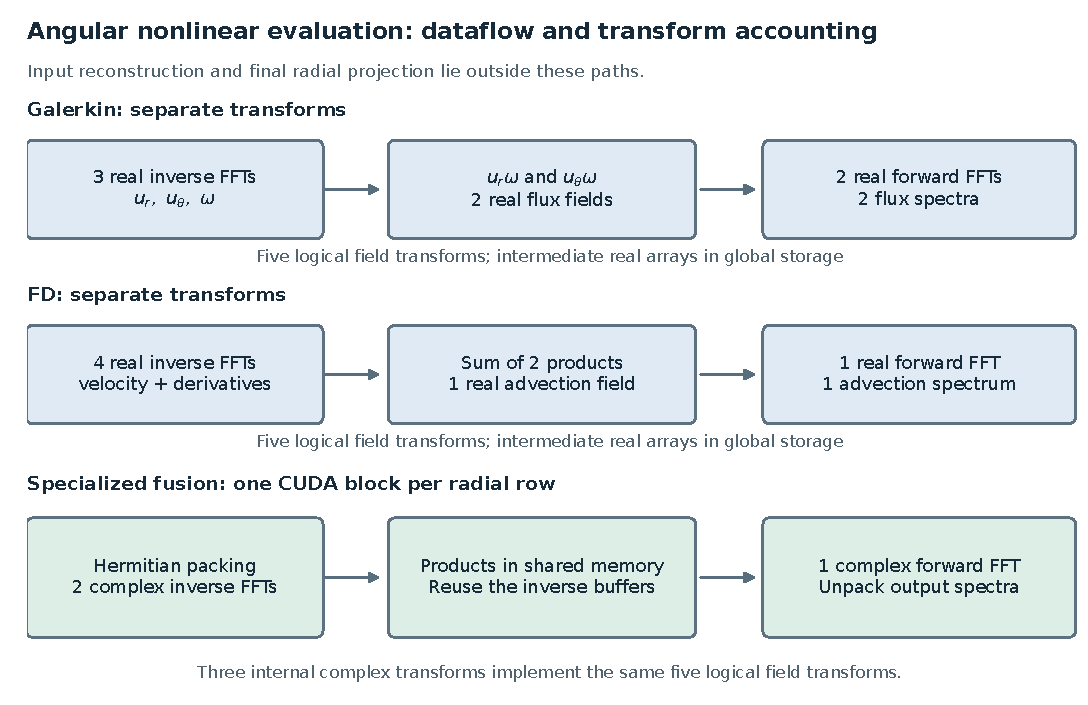
\includegraphics[width=\linewidth]{figures/nonlinear_pipeline.pdf}
\caption{The nonlinear operator boundary. The two discretizations retain their respective field products. Fusion combines the angular transforms, physical products, and packing in shared memory; radial reconstruction and projection lie outside the illustrated replacement. Five logical field transforms remain in both variants.}
\label{fig:operator-pipeline}
\end{figure}

\subsection{Packing identities and normalization}

Define the unnormalized forward and inverse transforms by
\begin{equation}
\label{eq:op-dft}
(\mathcal F_N v)_k=\sum_{j=0}^{N-1}v_j e^{-2\pi\mathrm{i}jk/N},\qquad
(\mathcal B_N A)_j=\sum_{k=0}^{N-1}A_k e^{2\pi\mathrm{i}jk/N}.
\end{equation}
Thus \(\mathcal B_N\mathcal F_N=N I\). The CUDA replacement follows the cuFFT convention\cite{r11}; it does not insert an additional \(1/N\). In the solver, the corresponding normalization already belongs to the following projection or FD right-hand side. Applying it in both locations would change the nonlinear equation, even if a standalone round-trip transform appeared correct.

For two separately Hermitian spectra \(A,B\), linearity gives
\begin{equation}
\label{eq:op-inverse-pack}
\mathcal B_N(A+\mathrm{i}B)=a+\mathrm{i}b,
\qquad a=\mathcal B_N A\in\mathbb R^N,\quad b=\mathcal B_N B\in\mathbb R^N.
\end{equation}
The negative modes must be reconstructed as \(\overline{A_k}+\mathrm{i}\overline{B_k}\). Conjugating the packed positive mode as a whole instead produces \(\overline{A_k}-\mathrm{i}\overline{B_k}\) and is incorrect. The packed sequence is generally not Hermitian. At zero frequency, and at Nyquist frequency for even \(N\), each original real-field coefficient has zero imaginary part.

After forming two real products \(g,h\), let \(Z=\mathcal F_N(g+\mathrm{i}h)\). Their separate spectra follow from
\begin{equation}
\label{eq:op-forward-pack}
G_k=\frac{Z_k+\overline{Z_{-k}}}{2},\qquad
H_k=\frac{Z_k-\overline{Z_{-k}}}{2\mathrm{i}}.
\end{equation}
The Galerkin implementation uses one packed inverse for the two velocities, one inverse for vorticity, and one packed forward for the two fluxes. The FD implementation packs the two velocities and the two derivatives separately, forms their dot product, and performs one forward transform. Consequently both use three internal complex transforms. This accounting is an implementation identity, not evidence of a factor \(5/3\) speedup: real cuFFT transforms exploit Hermitian redundancy already, and the packing, permutation, synchronization, and instruction costs must also be paid.

For a retained band \(|k|\le K\), quadratic products have support at most \(2K\). An aliased contribution into a retained mode would require \(|k+\ell N|\le2K\) for some nonzero integer \(\ell\). Since \(|k+\ell N|\ge N-K\), the strict condition \(N>3K\) excludes such a contribution. This is the standard retained-band dealiasing argument\cite{r13}. It does not imply that modes above \(K\) vanish in the product, nor does it remove radial quadrature error. The replacement preserves the original padded angular grid and truncation.

\subsection{Block mapping, synchronization, and memory traffic}

One 128-thread block handles one radial row. Two shared arrays of \(N\) complex doubles hold the packed inverse inputs and physical fields. The specialized lengths and factorizations are \(200=2^3 5^2\), \(225=3^2 5^2\), and \(243=3^5\). Their shared storage is respectively 6400, 7200, and 7776 bytes per block. These are the supported kernel instantiations; the code is not a general arbitrary-length FFT service.

Let the ordered radices be \(r_0,\ldots,r_{s-1}\), and express an input position using mixed-radix digits \(d_j\). The load permutation is
\begin{equation}
\label{eq:op-permutation}
p(i)=\sum_{j=0}^{s-1}d_j\frac{N}{\prod_{\ell=0}^{j}r_\ell},\qquad
i=\sum_{j=0}^{s-1}d_j\prod_{\ell=0}^{j-1}r_\ell.
\end{equation}
At a stage with previous-radix product \(m\) and current radix \(r\), disjoint butterflies combine positions separated by \(m\), after the appropriate twiddle multiplication. Each thread visits butterflies in strides of 128. A block barrier separates consecutive stages. This is a classical mixed-radix FFT construction; the project contribution is its specialized mapping within this operator boundary, not a new FFT factorization.

The complete sequence is: load the two packed inverse planes in permuted order; execute the inverse stages; retain each thread's one or two physical products in registers; synchronize all reads; overwrite the first shared plane with the permuted products; execute the forward stages; unpack and store the output half-spectra. The register retention and barrier before overwrite are necessary because another thread may still need the old inverse output. Omitting that barrier introduces a read/write race despite using a single block. Including initial-load and overwrite barriers, the number is \(2s+3\), or 13, 11, and 13 for the supported lengths.

The separate implementation materializes inverse physical arrays and forward product arrays in global memory. Counting writes and reads of these named arrays gives a nominal source-level reduction of \(80Nq\) bytes per nonlinear evaluation in either variant. For Galerkin, the count is \((3+3+2+2)Nq\) doubles; for FD it is \((4+4+1+1)Nq\) doubles. This is an access model for the named real arrays, not a bound on total eliminated device traffic. It excludes cache reuse, compiler behavior, library workspaces, and traffic still required for spectral input, flux output, and flux history. It must not be reported as measured DRAM traffic or converted directly into a bandwidth speedup.

Fusion also increases shared-memory use, register lifetimes, and per-block work. The specialized row count may expose too few blocks to saturate a GPU, while consumer hardware may have limited FP64 throughput. Therefore reduced temporary storage does not by itself establish whether the resulting kernel is bandwidth-bound, instruction-bound, or latency-bound. A roofline or occupancy conclusion would require hardware counters and controlled measurements not collected in this study.

\subsection{Floating-point limits and a guarded standalone extraction}

Equations~\eqref{eq:op-inverse-pack}--\eqref{eq:op-forward-pack} hold in exact arithmetic. In floating-point arithmetic, a packed channel of characteristic magnitude \(A\) can introduce an absolute perturbation on the scale of \(\epsilon A\) into a second channel of magnitude \(B\). The corresponding relative scale is \(\epsilon A/B\), before considering transform constants or cancellation. This is an explanatory scale estimate, not an error bound for this kernel. It explains why a combined-vector norm can hide a poor relative error in a weak output. Near-cancelling product sums require an additional absolute error scaled by the magnitudes of the uncancelled terms.

The revision extracts the original CUDA file and its existing CPU model without modifying their bytes, and adds a solver-independent harness with new NumPy and direct-convolution oracles. The input contract checks supported lengths, FP64 contiguous layouts, real endpoints, zero padding, finite data, and valid retained bandwidth. As a new engineering guard, the adapter rejects a pair of nonzero packed input spectra if the smaller per-row maximum magnitude is less than \(10^{-8}\) times the larger. The threshold is a conservative dispatch policy, not a sufficient condition for a relative-error theorem. Exactly zero channels instead require an absolute-error check. A production integration would need a verified unpacked fallback and a low-cost way to obtain the relevant scales; neither is claimed here. The frozen NS kernels and their qualification records are unchanged.

The harness was run on the local GPU for 36 fixed-state cases: three lengths, two variants, and six fixture classes per variant. The sixth class is a zero velocity channel for Galerkin and additive cancellation for FD, giving seven distinct labels across the two variants. It uses both an independent NumPy FFT oracle and an FFT-free retained-band convolution oracle; it also checks flux history and FD mean-buffer parity. For each output channel, the relative metric is the infinity-norm ratio \(\max_{i,k}|Y_{ik}-Y^{\rm ref}_{ik}|/\max_{i,k}|Y^{\rm ref}_{ik}|\), over all radial rows and half-spectrum modes, not a pointwise relative error. Ordinary cases attained a maximum channel-relative error of \(1.18\times10^{-15}\). The absolute diagnostic uses one common scale across channels: the maximum, over output channels and rows, of \(N\) times the sum of the products of the separate physical-field maximum magnitudes in each flux expression. Across all fixtures, the largest absolute error divided by this uncancelled scale was \(3.84\times10^{-16}\). Because this common scale can hide errors in a weak channel, it must be read together with the per-channel relative metrics. Deliberately reducing one velocity channel by \(10^{-10}\), after confirming rejection by the guard and explicitly overriding it for diagnosis, produced a maximum channel-relative error of \(4.98\times10^{-6}\). These rounded-up figures describe new synthetic verification, distinct from the earlier archived operator measurements. No new timing or NS trajectory was collected for this extraction. It is distributed as a local contribution candidate in the supplementary source package.

\subsection{Observation reduction and CPU kernels}

The probe operator evaluates six weighted sums, \(p_j=w_j^\top x+\ell_j(t)\). The old implementation assigned each sum to one thread. The replacement assigns a complete warp to each probe: lane \(\ell\) accumulates indices \(\ell+32m\), then five shuffle reductions combine lane values\cite{r18}. A block of 192 threads therefore covers all six probes. The arithmetic work remains linear in the frame length; the per-probe serial depth is reduced from roughly \(L\) to \(\lceil L/32\rceil+5\), ignoring instruction and memory costs. Snapshot copies, selected state pointers, and synchronization before advancing the state are preserved. Reordering additions changes rounding, so bitwise state preservation and numerical probe agreement are separate assertions. This common observation improvement is applied to both Galerkin and FD comparisons.

There are also project-local C implementations below the Python driver. The Galerkin contraction kernel places the angular mode in the contiguous inner loop and combines the same precontracted mass and flux projections. The buffered FD kernel applies already assembled narrow radial stencils, reuses working arrays, and forms physical products in place. A separate band solver applies cached real LAPACK factor data to interleaved complex right-hand sides. The FD build specifies optimization and AVX2 support while disabling fused multiply-add contraction; that compiler option alone does not certify SIMD utilization or a speedup. SciPy still provides selected FFTs or factorization services in these CPU variants. The project does not replace their algorithms or patch their source.

These implementations demonstrate genuine low-level changes, but their existence is not an isolated end-to-end timing result. Likewise, replacing the Python orchestration language with Rust would not directly reduce the device FFT work, retained rank, or compiled-kernel initialization. A language migration would be justified only by a measured host bottleneck or a reusable interface requirement. The current attribution distinguishes loop/layout changes from module import, compilation caching, and CUDA graph scheduling.

\subsection{Costs, amortization, and upstream scope}

For attribution, write the total cost as
\begin{equation}
\label{eq:cost}
\begin{aligned}
T_{\rm total}={}&T_{\rm start}+T_{\rm prepare}+N_{\rm nl}C_{\rm nl}\\
&+N_{\rm step}C_{\rm lin}+N_{\rm obs}C_{\rm obs}+T_{\rm finish}.
\end{aligned}
\end{equation}
The costs denote phase-weighted effective quantities, not an assertion that every step costs the same. Here \(C_{\rm lin}\) excludes the nonlinear and observation terms already counted. Time-grid optimization changes \(N_{\rm nl}\) and \(N_{\rm step}\); fusion changes \(C_{\rm nl}\); warp reduction changes \(C_{\rm obs}\); and preparation reuse or caching changes other terms. Their savings cannot be added across unrelated measurements or counted twice.

If a fraction \(f\) of an otherwise fixed execution is accelerated by a local factor \(s\), the corresponding ideal bound is \([1-f+f/s]^{-1}\). An additional initialization cost makes the gain smaller. More explicitly, let \(S_b,S_f\) be setup costs and \(B_b,B_f\) the costs of one otherwise matched repeated workload. Under genuine reuse of setup, the fused path wins after \(m\) repetitions only if
\begin{equation}
\label{eq:op-amortization}
m(B_b-B_f)>S_f-S_b.
\end{equation}
If each new process rebuilds or reloads the relevant state, setup is not a once-only term and this amortization model must be changed. The fixed-state event measurements and short-trajectory results in the next section illustrate precisely why the distinction matters. An explicit PTX cache also does not eliminate all driver JIT, loading, context, planning, or process-start costs.

The complete-solve clock includes construction, compilation or loading, transfers, FFT preparation, graph capture, advancement, observation, synchronization, download, and resource release. The new-process clock additionally includes interpreter startup, imports, and the prescribed supervision overhead. Neither clock can be replaced by isolated kernel events. Numerical qualification may use concurrent independent jobs, but latency comparison requires serialized GPU use and monitored external activity. Aggregate CPU utilization is not an accuracy-constrained performance metric.

Finally, the source audit found project-local application kernels and library calls, not an identified modification to borrowed cuFFT, cuFFTDx, SciPy, or LAPACK source. NVIDIA already provides FFT fusion and convolution examples, including comparisons with a cuFFT pipeline and optional LTO callbacks\cite{r17}. The plausible upstream contribution is therefore a new multifield FP64 inverse-transform--cross-product--forward-transform example, not a claim to have invented FFT fusion or repaired cuFFT. A useful proposal still requires an equivalently fused cuFFTDx implementation, a batched cuFFT baseline, matched precision and padding, first-use and repeated-use costs, and a clean build outside this machine. The local extraction has not satisfied those performance and portability requirements, has not established a new license grant or contribution certification, and has not been submitted as a PR\cite{r19}.

\subsection{Maintenance of the early steady-solver interface}
The dynamic replacement cited by the reviewer belongs to an early steady-cavity
control: its wrapper temporarily replaced
\path{rfm_v2_solver.trial_basis}, outside the final annular solver path.
We preserve the archived source hashes and provide a separate maintained package
with an explicit, solve-local basis factory. Omitting this argument preserves the
default behavior; the mapped-Legendre wrapper no longer changes module globals.
All seven CPU tests pass. Eight small configurations agree with the archived
functions in coefficients, Stokes matrices, and velocity, vorticity and other fields
at 25 independent points, using relative and absolute tolerances of $10^{-12}$.
Additional tests force concurrent factory overlap and check default calls after
factory and assembly exceptions. These establish interface compatibility and
state isolation for this change; they provide no new annular accuracy certificate,
GPU speed result, or thread-safety guarantee for arbitrary user-supplied factories.


\section{Experimental design and attribution protocol}
\label{sec:validation}

The experiments answer three different questions: whether a discretization reaches the prescribed physical accuracy, whether an implementation preserves that discretization, and whether a qualified implementation reduces complete solution time. These questions require different controls. A successful trajectory is evidence for numerical feasibility; a fast isolated operator is evidence about that operator; a complete paired timing campaign is required to establish a practical speed advantage. We retain these distinctions when reporting both successful and unsuccessful candidates.

\subsection{Problem, references, and independent reconstruction}

All main comparisons concern the finite annulus with $a=0.5$, $R=6$, $\nu=0.01$, and $T=72$. The final incident speed and cylinder diameter are both unity, giving $\mathrm{Re}=100$. The transverse pulse ends at $t=12$, whereas the observations extend to $t=72$. No reflection constraint is imposed, and neither the fields nor the probe series are shifted in time or aligned by wake phase. This is necessary because accumulated phase error is part of the approximation error for an initial-boundary-value problem.

The two frozen numerical references, denoted \texttt{angular\_fine} and \texttt{time\_fine} in the archive, resolve angular and temporal refinement separately within a finite-difference refinement chain. The chain increases the radial resolution from 384 to 448 intervals, angular truncation from 128 to 144, and step rate from 384 to 512. They are distinct numerical references, not two independently implemented continuum-solution certificates. Their combined late-time discrepancy is $0.0290144\%$. This is below the empirical reference allowance of $0.125\%$, one quarter of the candidate tolerance. It is above the $0.025\%$ allowance that the same rule would assign to a $0.1\%$ candidate tolerance. Consequently the current reference evidence supports the reported $0.5\%$ protocol, without establishing a certified continuum error or a tighter accuracy target.

Evaluation is performed after reconstructing every method on the same physical grids. For reconstruction grid $G$, checkpoint $t$, and its physical weights, define
\begin{equation}
\label{eq:field-errors}
 E_u(G,t)=\frac{\|\boldsymbol u-\boldsymbol u_{\rm ref}\|_G}{\|\boldsymbol u_{\rm ref}\|_G},\qquad
 E_\omega(G,t)=\frac{\|\omega-\omega_{\rm ref}\|_G}{\|\omega_{\rm ref}\|_G}.
\end{equation}
The measure is $r^2\,ds\,d\theta$, and the velocity norm combines both polar components. Each quantity is checked over the full annulus and over $r\leq2.5$. The reconstruction grids use 123, 129, and 144 radial points and respectively 433, 449, and 457 shifted angular points. They differ from the solver quadrature and FFT grids. Their construction and the 19 physical checkpoint times are listed in Appendix~\ref{sec:app-setup}. Taking the maximum across grids reduces dependence on an individual sampling pattern, but remains a finite set of discrete tests.

There are 19 reference-scored physical checkpoints from $t=0.5$ to $72$. A piecewise schedule saves two additional states immediately after the bridge for implementation comparison; the archive therefore distinguishes 19 physical checkpoints from 21 saved implementation checkpoints. Six probe histories, transverse velocity and vorticity at three downstream positions, contain 577 equally spaced times, including the zero initial value. The implementation tolerance against the CPU trajectory of the same discretization is $10^{-5}$ for the field and complete probe-series comparisons. The wake checker additionally verifies sustained alternating signs. Neither a plausible shedding frequency nor a visually similar wake substitutes for the field-error tests.

\subsection{A safeguard against compensating errors}

For a piecewise schedule, the constant-step control uses the same space, seed, geometry, and quadrature. Let $v$ be this control, $w$ the piecewise candidate, and $z$ a reference, all evaluated in the same weighted norm. Define $b=\|v-z\|_G/\|z\|_G$ and $d=\|w-v\|_G/\|v\|_G$. Then
\begin{equation}
\label{eq:triangle-guard}
 \frac{\|w-z\|_G}{\|z\|_G}
 \leq b+d\frac{\|v\|_G}{\|z\|_G}
 \leq b+(1+b)d.
\end{equation}
Both the direct error and $b+(1+b)d$ must be at most $0.005$. Using $b+d$ would incorrectly ignore the different denominators. The bound is evaluated for each prescribed field, region, grid, checkpoint, and reference, before taking maxima. It prevents a candidate from qualifying solely because the schedule error cancels part of its constant-step error. It is a rigorous relation between these discrete fields, not an a posteriori bound against the exact PDE solution.

This extra test can reject a candidate whose direct error passes. For high-resolution Legendre34, the piecewise direct field score is approximately $0.481690\%$, but the triangle safeguard is $0.509600\%$. Its constant-step variant remains eligible. Keeping that cheaper deterministic alternative is essential: applying a common accuracy target does not require every method to use an identical schedule when the question is minimum cost at that target.

\subsection{Controlled comparisons and computational environment}

Table~\ref{tab:fairness} separates the effects being compared. A same-rank comparison controls algebraic dimension but does not prove equal approximation power for all flows. A comparison of the least expensive qualifying configurations instead permits different ranks and schedules. Both are useful, and their conclusions must be labeled accordingly. The finite-difference baseline uses fourth-order radial spatial differences and the same second-order SBDF2 time family; ``fourth order'' does not describe its time discretization.

\begin{table}[tbp]
\centering\small
\caption{Comparison matrix and the effect each contrast can identify. All physical comparisons retain the same boundary-value problem and error criteria.}
\label{tab:fairness}
\begin{tabularx}{\linewidth}{@{}p{0.21\linewidth}XX@{}}
\toprule
Contrast & Held fixed & Quantity allowed to change \\
\midrule
RFM / Legendre at equal rank & $K,q$, retained rank, schedule, shared kernels and runtime policy & Trial functions and resulting approximation error \\
Accuracy-matched spaces & Reference, field and probe tests, runtime policy & Rank and qualified schedule; actual rank reported per seed \\
Constant / piecewise & Same trial space, seed, $K,q$ and observation protocol & Step schedule and associated phase preparation \\
cuFFT / fused operator & Input state, precision, retained spectrum, normalization and output definition & Transform implementation and temporary storage \\
Serial / warp observation & State evolution and probe weights & Floating-point summation order and observation cost \\
First use / cache hit & Solver, artifacts, accuracy criteria and fresh-process entry & Explicit compilation-artifact availability \\
Galerkin / FD & Physical problem, accuracy target, observation and runtime policies & Spatial discretization and its qualified resolution \\
\bottomrule
\end{tabularx}
\end{table}

The recorded experimental machine and software are summarized in Table~\ref{tab:hardware}. The numerical backend uses FP64 CUDA kernels and cuFFT through a native interface. The CPU reference and host preparation use NumPy and SciPy. A compatibility probe also exercised cuBLAS, but the native Galerkin march uses project-specific projection kernels; cuBLAS should not be credited as the production projection backend.

\begin{table}[tbp]
\centering\small
\caption{Recorded environment of the archived Windows experiments. Version labels describe the measured environment, not a recommendation to use the latest available release.}
\label{tab:hardware}
\begin{tabularx}{\linewidth}{@{}lX@{}}
\toprule
Component & Recorded value \\
\midrule
CPU & AMD Ryzen 9 9955HX, 16 cores, 32 logical processors \\
GPU & NVIDIA GeForce RTX 5060 Laptop GPU; compute capability 12.0 \\
Operating system / driver & Windows 11, build 26200; NVIDIA 596.13, WDDM \\
Scientific runtime & Python 3.13.5; NumPy 2.2.6; SciPy 1.16.3 \\
Main CUDA components & CUDA 11.8 NVRTC and cuFFT; driver API version 13020 \\
Precision and host threading & FP64 arithmetic; one BLAS thread in controlled comparisons \\
Main observation / nonlinear path & Warp probe reduction / original batched cuFFT \\
\bottomrule
\end{tabularx}
\end{table}

Independent qualification reconstruction can use several CPU workers while a single owner captures GPU trajectories. Those elapsed times are excluded from method rankings. The intended latency experiment instead runs one GPU solve at a time with fixed affinities, an identical runtime policy, and sampled external-load checks. Low total CPU utilization during this experiment is expected: one controlled host core is only one of 32 logical processors. Concurrent throughput is a different objective and was not measured by this campaign.

\section{Accuracy, trial-space size, and nonlinear workload}
\label{sec:accuracy-results}

\subsection{Qualified configurations and retained ranks}

Table~\ref{tab:configurations} lists the main configurations. The RFM and Legendre suffixes denote input basis counts, whereas the retained rank is obtained after enrichment, scaling, and truncation. The mean block retains rank 30 throughout. A finite-difference label $n$ counts radial intervals, giving $n+1$ nodes and $n-1$ interior unknowns per angular mode. These interval counts are not directly comparable to a Galerkin retained rank.

\begin{table}[tbp]
\centering\small
\caption{Spatial configurations and eligible step-rate schedules. An arrow denotes the change at $t=8$.}
\label{tab:configurations}
\begin{tabularx}{\linewidth}{@{}Xcl>{\raggedright\arraybackslash}p{0.27\linewidth}@{}}
\toprule
Configuration & Rank & $K/q$ & Step rate \\
\midrule
Mid RFM37 & 39 & $72/66$ & $128$ or $128\to112$ \\
Mid Legendre35 & 39 & $72/66$ & $128$ or $128\to112$ \\
High RFM41 & 40 & $80/76$ & $152$ or $152\to136$ \\
High RFM35 & 38 or 39 & $80/76$ & $152$ or $152\to136$ \\
High Legendre36 / 35 & 40 / 39 & $80/76$ & $152$ or $152\to136$ \\
High Legendre34 & 38 & $80/76$ & $152$ only \\
FD176 dense / FD184 banded & --- & $K=80$ & $128$ throughout \\
\bottomrule
\end{tabularx}
\end{table}

There are 39 unique numerical identities, each evaluated under two explicit compilation-cache policies, for 78 GPU trajectories through $T=72$. Every trajectory passed the registered physical, implementation, and wake criteria. Within each of the 39 cache-policy pairs, saved states, times, and probe arrays were bitwise identical. These are 39 numerical configurations reproduced under two policies, not 78 independent random-feature samples.

\begin{table}[tbp]
\centering\small
\caption{Worst errors by method and schedule, in percent. Each entry includes all registered seeds, both cache policies, the references, reconstruction grids, and checkpoints. Velocity and vorticity include full-domain and near-field checks.}
\label{tab:accuracy}
\begin{tabularx}{\linewidth}{@{}Xlrrr@{}}
\toprule
Configuration & Schedule & Velocity & Vorticity & Guard \\
\midrule
RFM37 / K72 & Uniform & 0.02943 & 0.40960 & — \\
RFM37 / K72 & Piecewise & 0.04467 & 0.43168 & 0.47865 \\
Leg35 / K72 & Uniform & 0.02676 & 0.44207 & — \\
Leg35 / K72 & Piecewise & 0.04104 & 0.45665 & 0.49773 \\
FD176 / K80 & Uniform & 0.10497 & 0.40876 & — \\
RFM41 / K80 & Uniform & 0.01819 & 0.33189 & — \\
RFM41 / K80 & Piecewise & 0.02595 & 0.34034 & 0.36867 \\
Leg36 / K80 & Uniform & 0.01613 & 0.36205 & — \\
Leg36 / K80 & Piecewise & 0.01972 & 0.36634 & 0.39405 \\
Leg35 / K80 & Uniform & 0.01896 & 0.41520 & — \\
Leg35 / K80 & Piecewise & 0.02235 & 0.41914 & 0.44722 \\
FD184 / K80 & Uniform & 0.07900 & 0.30652 & — \\
RFM35 / K80 & Uniform & 0.01935 & 0.42818 & — \\
RFM35 / K80 & Piecewise & 0.02309 & 0.43245 & 0.46494 \\
Leg34 / K80 & Uniform & 0.02301 & 0.47754 & — \\
\bottomrule
\end{tabularx}

\end{table}

Across the full cohort, the maximum direct physical error is $0.477543\%$, and the maximum safeguard is $0.497730\%$. The latter leaves only approximately $0.002270$ percentage points below the $0.5\%$ limit. It is a measured acceptance margin rather than evidence of robustness to changes in Reynolds number, boundary conditions, or floating-point environment. The largest velocity error across full and near fields is $0.10497\%$; thus the tightest constraints arise from vorticity. This explains why velocity-only validation would have admitted a substantially weaker test.

The largest GPU-to-CPU field error is $3.5721\times10^{-6}$ and the largest probe-series error is $3.8792\times10^{-6}$, both below $10^{-5}$. These maxima correspond to the finite-difference control. For the final rank-expanded cases lacking a historical serial-observer control, the qualification still uses the registered CPU and reference comparisons; an unavailable earlier observer pairing is not silently treated as additional evidence.

\subsection{Seed variation and the deterministic alternative}

The five RFM seeds are fixed before the final qualification: 7331, 7687, 8011, 8353, and 9041. Table~\ref{tab:seeds} exposes a confounding factor that is hidden if only the input label RFM35 is reported. Four seeds retain 38 radial functions and one retains 39. The smaller vorticity error for seed 8353 therefore occurs in a larger retained space. It cannot be attributed solely to a better draw of equal-dimensional features. Five fixed seeds also do not support a probabilistic guarantee over the feature distribution.

\begin{table}[tbp]
\centering\small
\caption{High-resolution RFM35 by seed. Errors and safeguards are percentages, recomputed from the archived qualification scores; the two cache policies give the same arrays.}
\label{tab:seeds}
\begin{tabularx}{\linewidth}{@{}rrXXX@{}}
\toprule
Seed & Rank & Constant-step $E_\omega$ & Piecewise $E_\omega$ & Piecewise safeguard \\
\midrule
7331 & 38 & 0.427183 & 0.431520 & 0.463945 \\
7687 & 38 & 0.427945 & 0.432246 & 0.464707 \\
8011 & 38 & 0.428183 & 0.432451 & 0.464943 \\
8353 & 39 & 0.378031 & 0.383875 & 0.414801 \\
9041 & 38 & 0.427611 & 0.431910 & 0.464372 \\
\bottomrule
\end{tabularx}
\end{table}

The rank-38 Legendre34 constant-step method also qualifies. Thus the evidence supports compact random-feature and deterministic polynomial spaces at this tolerance, but does not establish that randomness is necessary for compactness. A fair cost comparison must retain Legendre34 even though its piecewise variant fails, and must include Legendre35 and Legendre36 to separate equal-rank from accuracy-matched contrasts. High-resolution Legendre33 fails the $T=72$ accuracy tests; a short-horizon pass is insufficient for promotion. The reduced mid-resolution RFM35 screen also does not replace the registered five-seed RFM37 cohort.

\subsection{Wake dynamics and the cost removed by scheduling}

Figures~\ref{fig:annulus-wake} and \ref{fig:wake-probes} show the retained asymmetry and alternating shedding. The images display a local window, while scoring covers the prescribed full and near domains. The probe plot combines qualified trajectories and a fine reference for physical interpretation. Its curves are not from a single isolated timing batch and are not used to estimate errors by inspection.

\begin{figure}[tbp]
\centering
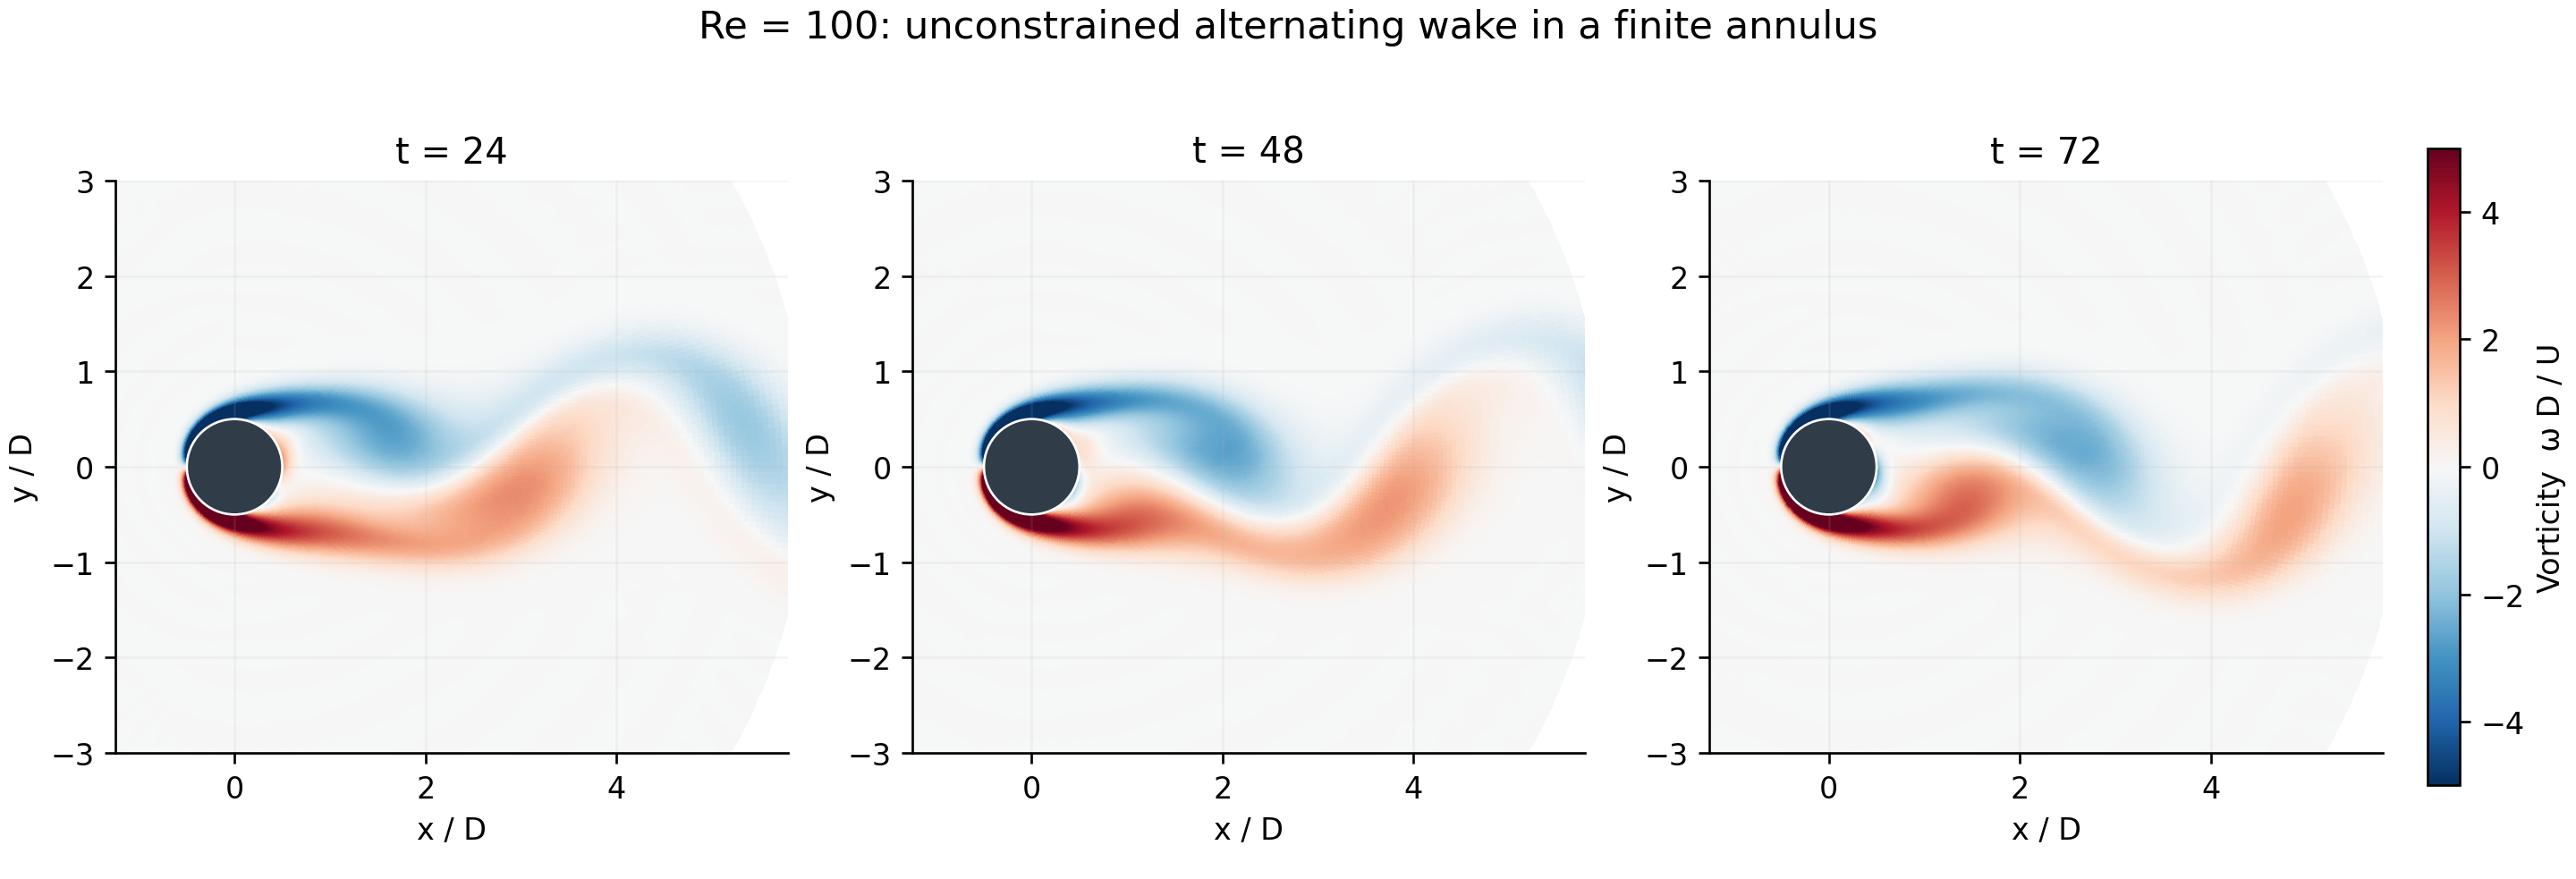
\includegraphics[width=\linewidth]{figures/finite_annulus_vorticity.png}
\caption{Vorticity at $t=24$, $48$, and $72$ for one qualified RFM41 trajectory, without imposed reflection symmetry. The common color scale covers a local view of the annulus; the outer radius is 6.}
\label{fig:annulus-wake}
\end{figure}

\begin{figure}[tbp]
\centering
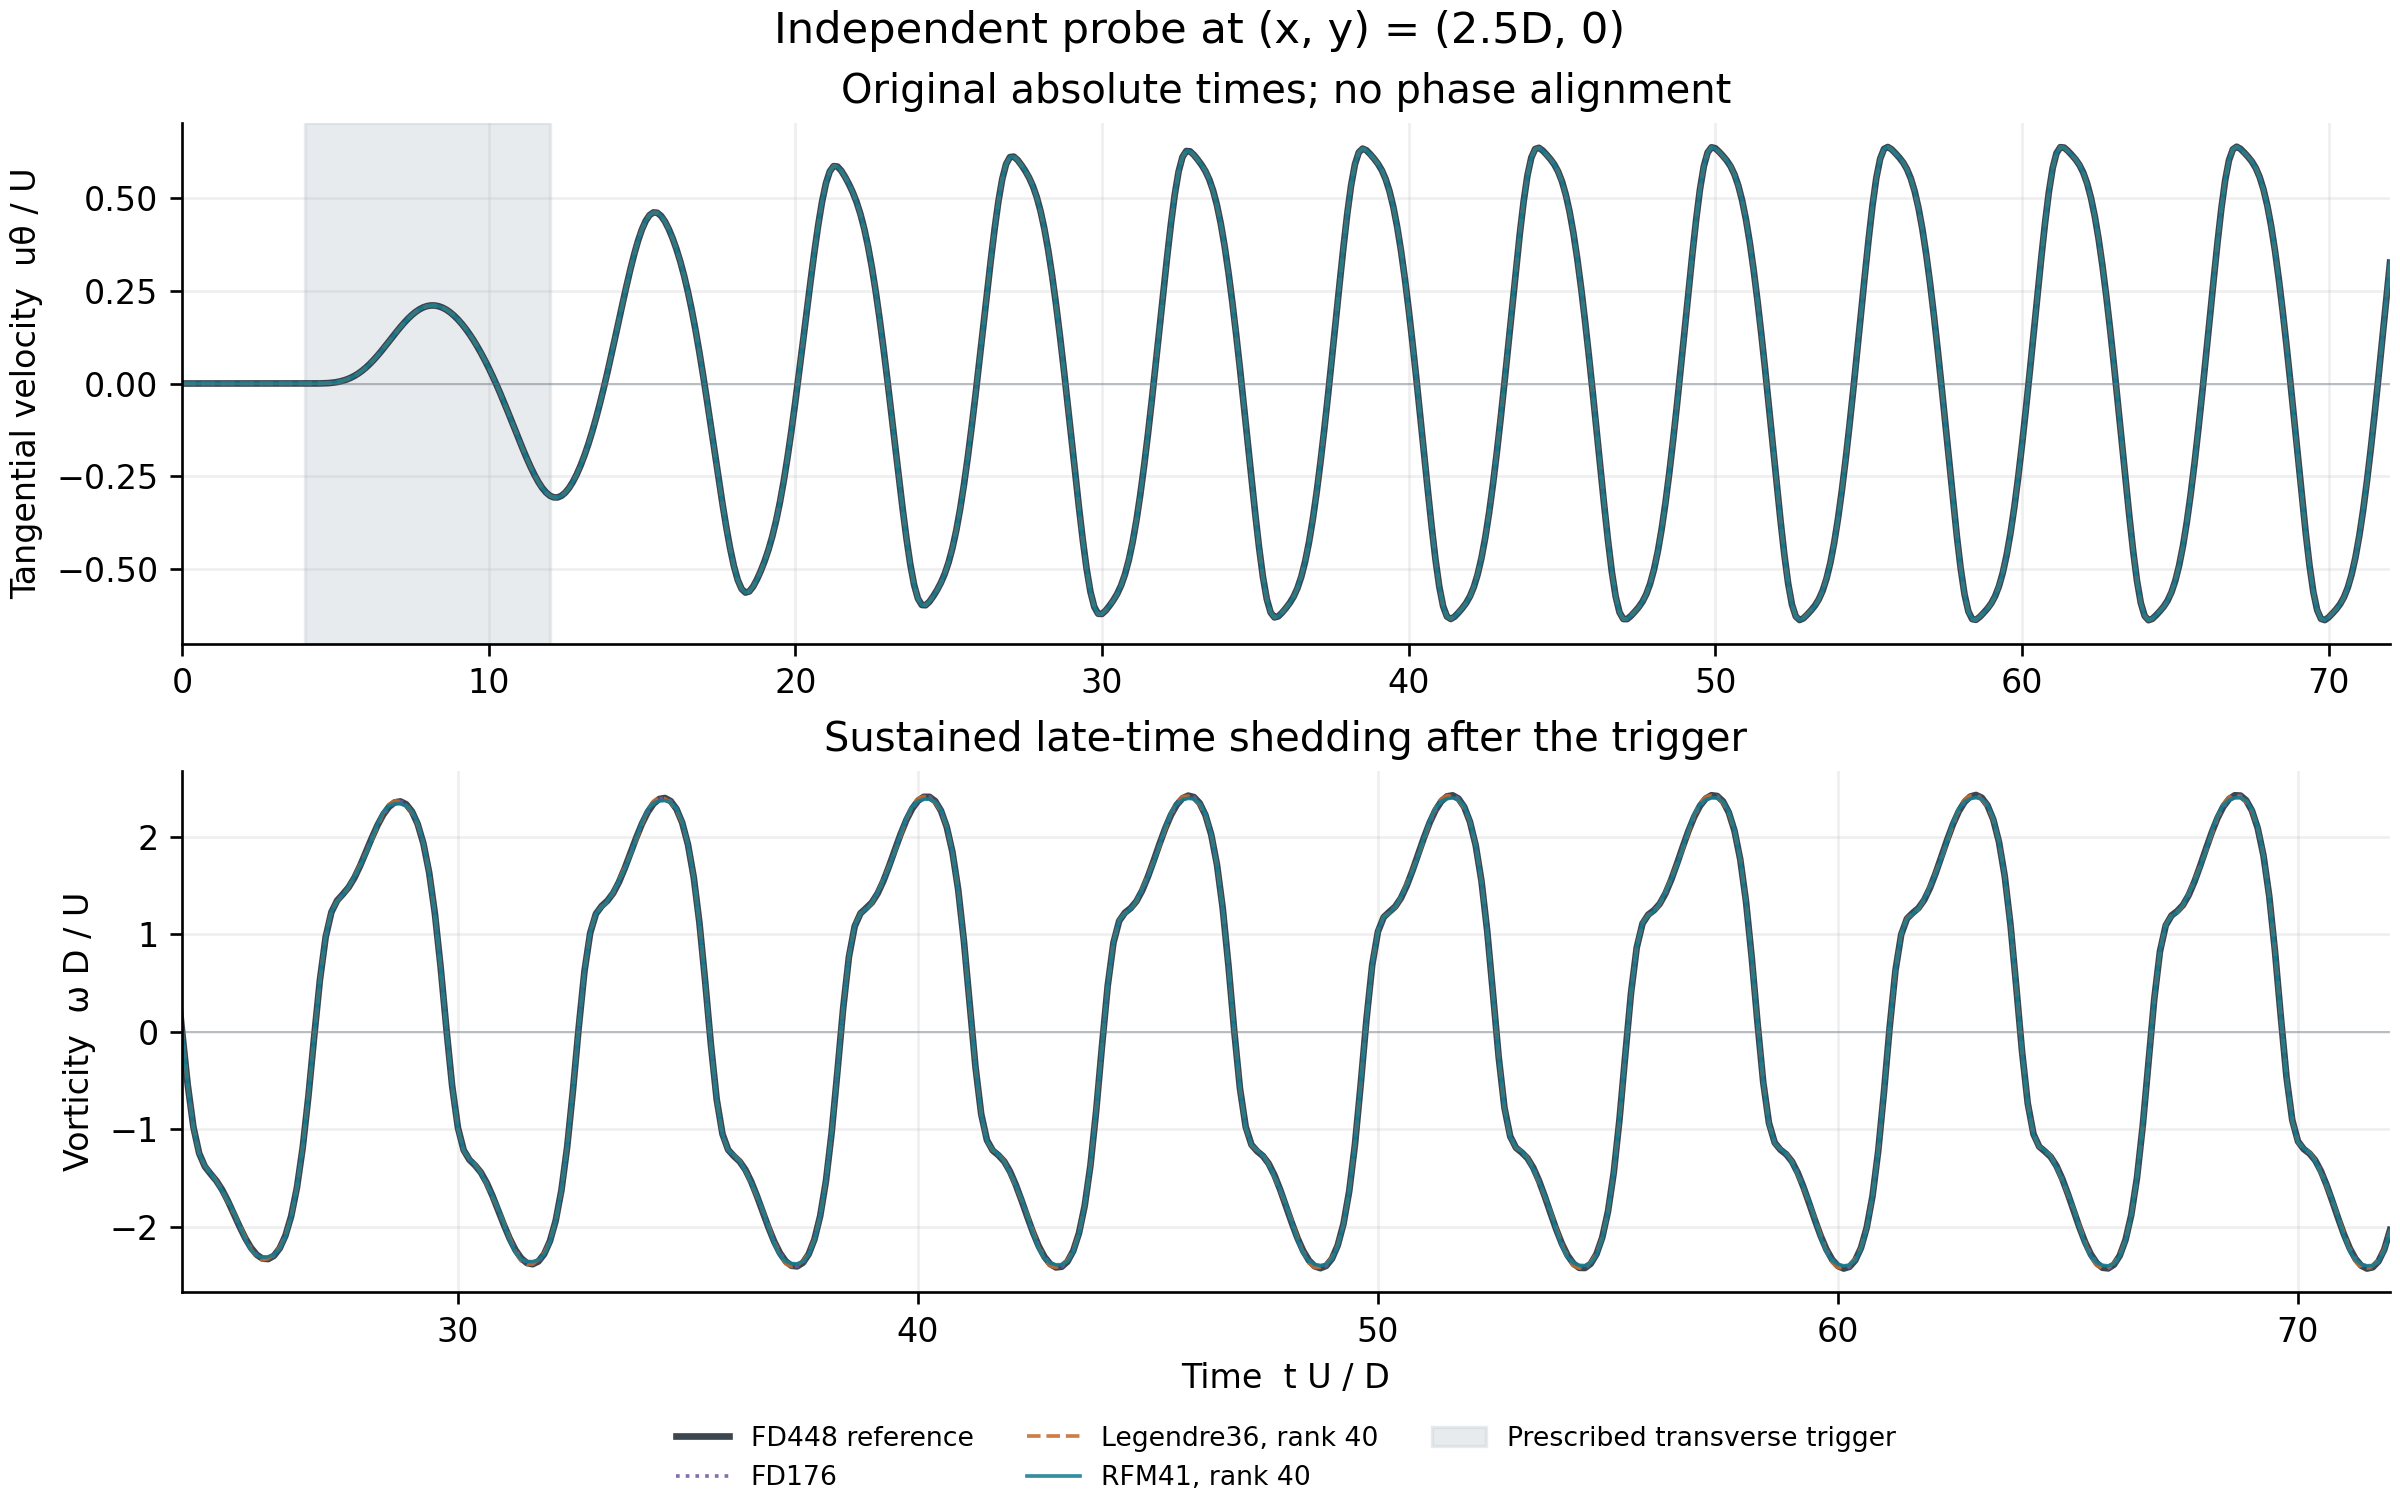
\includegraphics[width=0.88\linewidth]{figures/unshifted_wake_probes.png}
\caption{Unshifted probe histories at $x=2.5D$, $y=0$. Alternating shedding persists after the triggering pulse. RFM41 and FD176 are qualified GPU trajectories, Legendre36 is its corresponding CPU qualification, and FD448 is the reference.}
\label{fig:wake-probes}
\end{figure}

\begin{table}[tbp]
\centering\small
\caption{Recorded nonlinear evaluations for the two piecewise schedules. Both switch at $t=8$ and end at $T=72$.}
\label{tab:workload}
\begin{tabularx}{\linewidth}{@{}Xrrr@{}}
\toprule
Step-rate schedule & Constant step & Piecewise & Reduction \\
\midrule
$128\to112$ & 9,215 & 8,191 & 1,024 ($11.11\%$) \\
$152\to136$ & 10,943 & 9,919 & 1,024 ($9.36\%$) \\
\bottomrule
\end{tabularx}
\end{table}

The counts in Table~\ref{tab:workload} are read from runtime metadata rather than inferred from a nominal order label. Over the remaining 64 time units, reducing the step rate by 16 removes 1,024 steps; the recorded nonlinear counters differ by exactly the same amount. This saving applies to both RFM and Legendre. Reducing retained radial rank does not reduce $q$ or the angular FFT length in these experiments, and therefore does not additionally remove FFTs from each nonlinear evaluation. The work count is an algorithmic saving, while its conversion into elapsed time depends on preparation, linear algebra, observation, and runtime costs.

\section{Additional ablations, error decomposition, and switch sensitivity}
\label{sec:review-experiments}

This section reports 20 new CPU trajectories for the revision: 16 ablation/control runs and four delayed-switch runs. The original 78 GPU qualification records remain frozen. The additional comparisons use the existing two references and physical checkpoints; passing their field tests does not automatically confer promotion under the full probe and GPU-implementation protocol. Concurrent CPU durations are excluded from speed rankings.

\subsection{Additional ablation of frequency jitter and nonzero-mode layers}
\label{sec:review-ablation}
We fixed two configurations,
$(m,K,q,\Delta t^{-1})=(37,72,66,128)$ and $(41,80,76,152)$,
before executing a two-by-two ablation: registered random paired-frequency
jitter $\xi_j\sim U[0.2,0.8]$ versus fixed midpoints $\xi_j=0.5$, and six
nonzero-mode analytic outer-layer features present versus absent.
The random cells use the five registered seeds (7331, 7687, 8011, 8353, 9041).
Each deterministic cell has one unique trajectory; unused seeds are not counted
as replicates. All cells retain the same 24 mean-mode functions, six mean-mode
layers, quadrature, and time step. Adapter checks confirm bitwise equality of
the mean-mode discretization arrays and implicit operators across the four cells.

We computed 16 new CPU trajectories to $T=72$: 14 ablation trajectories and
two enriched-random CPU controls. Ten frozen enriched-random GPU trajectories
were reused and independently rescored. Every trajectory was evaluated at the
same 19 physical checkpoints on three grids against both fine FD references,
using velocity and vorticity errors over the full domain and $r\leq2.5$.
All four errors must be at most 0.5\%.
Table~\ref{tab:review-ablation} gives maxima over seeds, times, grids, and references.
All 16 CPU runs completed without numerical failure; the 12 trajectories without
nonzero-mode layers failed the accuracy gate. The two CPU controls differ from
the archived GPU fields by less than $2.0\times10^{-10}$ in the worst field metric.

\begin{table}[htbp]
\centering\small
\caption{Additional CPU accuracy ablation. Errors are percentages. Pass counts
exclude the two separate CPU controls. Random rows report the worst of five
seeds; midpoint rows contain one deterministic configuration.}
\label{tab:review-ablation}
\begin{tabular}{lrrrrrr}
\hline
Configuration & Rank & $e_u$ & $e_\omega$ & $e_{u,\mathrm{near}}$ & $e_{\omega,\mathrm{near}}$ & Pass \\
\hline
Mid, Random+layer & 39 & 0.0294 & 0.4096 & 0.0251 & 0.2100 & 5/5 \\
Mid, Midpoint+layer & 39 & 0.0293 & 0.4092 & 0.0249 & 0.2097 & 1/1 \\
Mid, Random/no layer & 34 & 19.4054 & 73.8980 & 26.4854 & 48.6306 & 0/5 \\
Mid, Midpoint/no layer & 34 & 19.3644 & 73.7836 & 26.4397 & 48.5825 & 0/1 \\
High, Random+layer & 40 & 0.0182 & 0.3319 & 0.0148 & 0.1799 & 5/5 \\
High, Midpoint+layer & 40 & 0.0181 & 0.3312 & 0.0147 & 0.1794 & 1/1 \\
High, Random/no layer & 35 & 18.7540 & 72.0115 & 25.7262 & 47.7640 & 0/5 \\
High, Midpoint/no layer & 35 & 18.7060 & 71.8705 & 25.6678 & 47.6945 & 0/1 \\
\hline
\end{tabular}
\end{table}

Both midpoint-plus-layer configurations pass, with errors comparable to the
random enriched cells. These data therefore do not establish randomness as
necessary for the observed accuracy. With raw $m$ and the SVD cutoff fixed,
removing the nonzero-mode layers reduces retained rank from 39/40 to 34/35 and
produces large velocity and vorticity errors; the mean rank remains 30.
The compact configurations depend strongly on analytic outer-layer enrichment,
but this design does not separate enrichment geometry from the increased
effective dimension. It is not an equal-rank enrichment ablation, and only one
deterministic frequency design was tested. All four error maxima for both
deterministic no-layer configurations occur at $T=72$. Their maximum vorticity
errors for $t\leq16$ are 2.820\% and 2.592\%, growing to 73.784\% and 71.871\%
at later times. The large errors therefore are not solely a consequence of a
near-zero startup reference field; the mechanism of error amplification is
not established by these data. A subsequent construction-only check increased raw $m$ to
41, 45, 49, 53, 57, and 61 while retaining bandwidth 62, quadrature, and the
SVD cutoff. Both resolutions produced ranks 35, 35, 36, 36, 36, and 36,
respectively, never recovering rank 39 or 40. We therefore did not add a
purported equal-rank $T=72$ control or tune the bandwidth/cutoff after failure.
Concurrent CPU elapsed times are
diagnostic only: they provide neither isolated timing nor new GPU speedup
evidence, and do not extend the original 78 GPU qualification trajectories.

\subsection{Matched-time radial and angular error diagnostics}
\label{sec:review-profiles}

The maximum errors in the qualification tables need not occur at the same time, grid, or reference. We therefore reanalyse the hash-bound CPU controls corresponding to the qualified high-resolution RFM41 (seed 7331), Legendre36, and FD184 trajectories. The first two use the original $t_s=8$ schedule and retain the same nonzero-mode rank 40. The uniform RFM41 and Legendre36 controls are also included in the machine-readable results. Both existing FD448/$K=144$ references are reconstructed: \texttt{angular\_fine} uses rate 384 and \texttt{time\_fine} rate 512. No reference or candidate is integrated for this analysis. All 19 physical times are retained; the figures show the common times $8,24,48,72$ against \texttt{time\_fine}. There is no phase alignment.

Let $e_f$ be the velocity-vector or scalar-vorticity error and let $\langle\cdot\rangle_\theta$ denote the angular mean. For the existing layer144 radial nodes and physical-area weights $w_i$, define
\input{equations/review_profile_norm.tex}
This normalization avoids dividing by a locally vanishing field. For real fields represented by nonnegative Fourier modes, the angular error contribution is
\input{equations/review_modal_error.tex}
For velocity, squared component magnitudes are summed in the polar representation $(u_r,u_\theta)$. The integrated vector-error energy is invariant under the pointwise orthogonal change to Cartesian components, but its allocation among angular modes depends on that representation; the displayed velocity spectrum is therefore a polar-component spectrum. Hence the weighted mean of $P_f^2$ and the sum of $Q_{f,k}^2$ both give the squared relative field error. The exact angular Parseval calculation agrees with the original layer144 physical-grid score to $2.13\times10^{-17}$ in 380 checks. Modes above the candidate cutoff $K=80$ contain the common unresolved reference tail, not additional candidate degrees of freedom.

\begin{figure}[htbp]
\centering
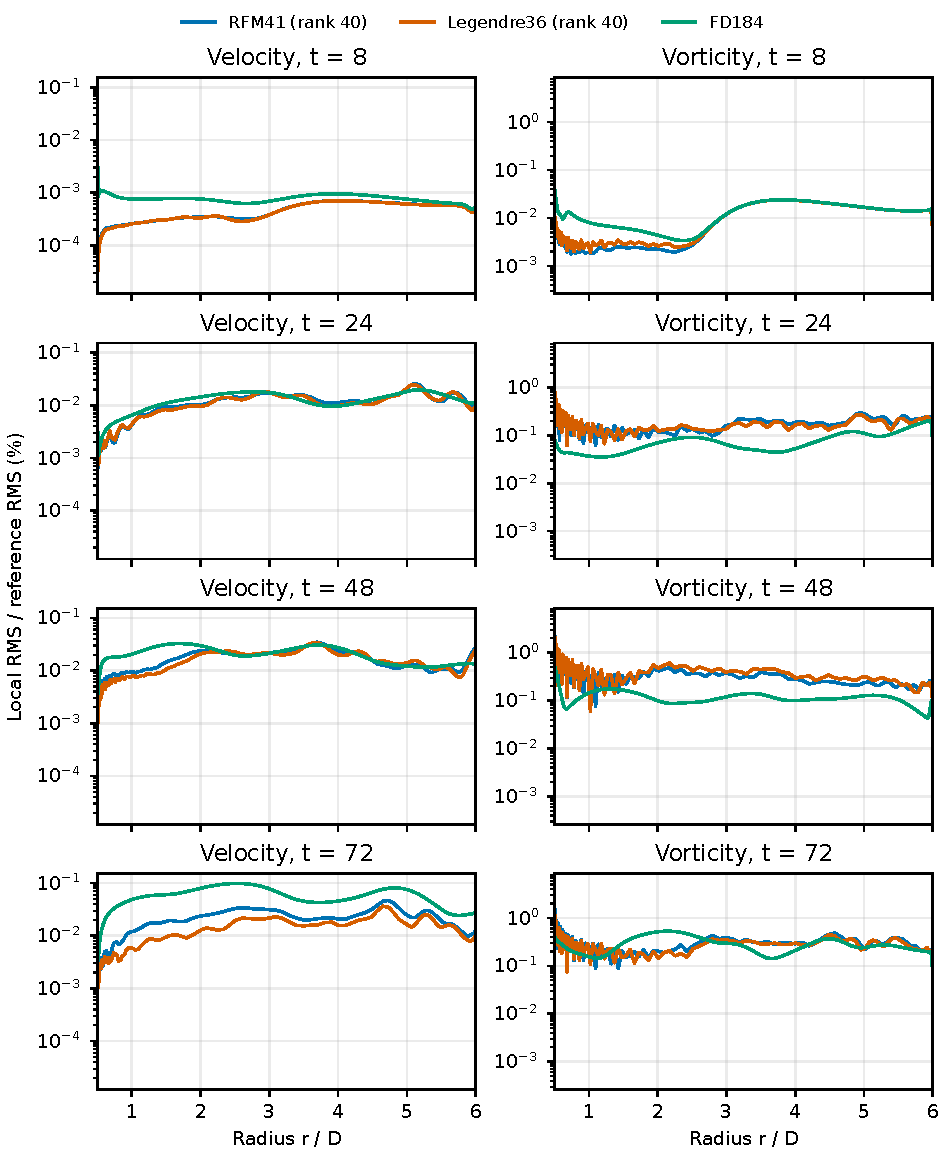
\includegraphics[width=\linewidth]{figures/review_radial_errors.pdf}
\caption{Matched-time radial error profiles $100P_f$ against the existing time-fine reference. RFM41 uses seed 7331. Galerkin curves use $t_s=8$; FD184 retains its qualified schedule. Curves share the same reference and times within each panel. The plotted quantity is a local angular RMS normalized by a global reference RMS, rather than a pointwise relative error.}
\label{fig:review-radial-errors}
\end{figure}

\begin{figure}[htbp]
\centering
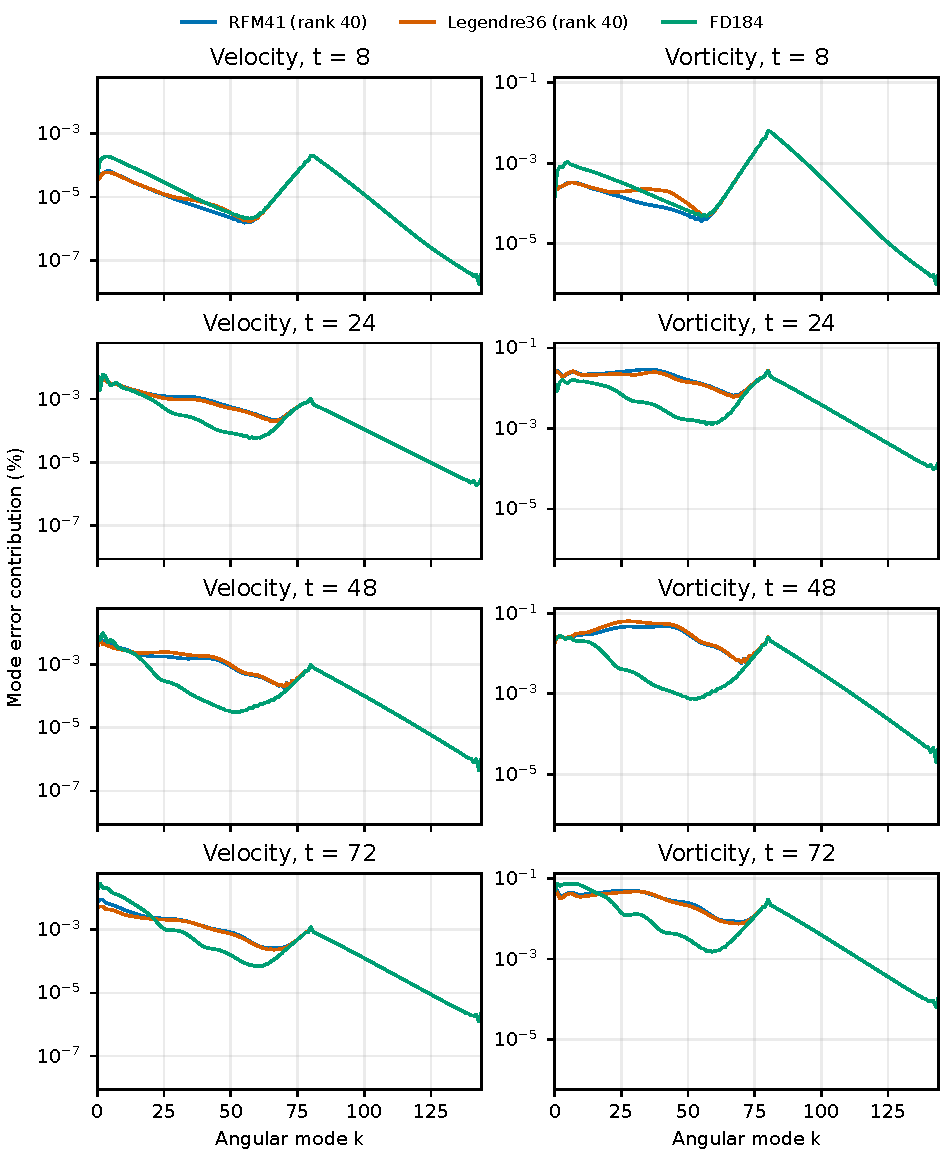
\includegraphics[width=\linewidth]{figures/review_angular_errors.pdf}
\caption{Angular error contributions $100Q_{f,k}$ for the same trajectories and times as Figure~\ref{fig:review-radial-errors}. Contributions combine in quadrature; they are not independently normalized modewise errors. The common tail above mode 80 reflects the finer reference spectrum.}
\label{fig:review-angular-errors}
\end{figure}

The original maxima are not a simultaneous ranking. For this RFM seed, the full-domain velocity and vorticity maxima occur at $t=72$ and $60$; the corresponding Legendre maxima occur at $60$ and $54$. In contrast, at the same $t=48$ and on layer144, RFM41, Legendre36, and FD184 have velocity errors $0.01886\%$, $0.01842\%$, and $0.02053\%$, but vorticity errors $0.29438\%$, $0.35509\%$, and $0.11317\%$. Thus even a simultaneous velocity ranking does not determine the vorticity ranking. Curl depends on first derivatives of velocity; an $L^2$ velocity comparison alone does not control their error. This observation is consistent with the measured spectra: at $t=72$, modes $k\le8$ contain $84.24\%$ of FD184's squared velocity-error norm, whereas modes $25\le k\le80$ contain $47.72\%$ of RFM41's squared vorticity-error norm, compared with $5.45\%$ for FD184.

The radial localization also requires qualification. At $t=72$, $61.14\%$ of RFM41's squared vorticity-error norm lies at $r\ge4$, but only $1.37\%$ lies at $r\ge5.9$. The observed error is therefore not confined to the narrow outermost layer. These diagnostics localize error in the full evolved solutions. They do not identify a causal benefit of the layer basis, or separate radial approximation, time discretization, boundary treatment, and reference uncertainty. The accompanying controlled ablation addresses basis attribution; the present figures alone do not.

\subsection{A CPU sensitivity experiment at $t_s=12$}
\label{sec:review-switch}

Revision 3 added four actual CPU trajectories through $T=72$: RFM37 and Legendre35 at rates $128\to112$, and RFM41 and Legendre36 at $152\to136$, switching at $t_s=12$ instead of 8. RFM uses seed 7331; the deterministic controls retain their original configurations. The generic CPU phase clock already accepts an explicit switch time. Its default observation list contains the old $t_s=8$ bridge instants, so this driver supplies the 19 common physical times explicitly. The underlying solver and archived data are unchanged. Four workers each use one BLAS thread; their elapsed times are not isolated performance evidence. Existing uniform and $t_s=8$ CPU controls are reused, rather than rerun or counted as new experiments.

All four new trajectories match the corresponding uniform CPU states exactly at the saved times $t\le12$. Both full-domain and near-field velocity and vorticity pass the $0.5\%$ threshold on all three grids against both frozen references; the per-cell triangle safeguard relative to the matching uniform control also passes, and alternating probe signs persist. Table~\ref{tab:review-switch12} reports full-domain field maxima separately from the worst safeguard across all four metrics. These are one-seed sensitivity results, not a new five-seed GPU qualification.

\begin{table}[htbp]
\centering\small
\begin{tabular}{llrrrr}
\hline
Configuration & Schedule & $E_u$ (\%) & $E_\omega$ (\%) & Guard (\%) & $N_{\rm nl}$\\
\hline
RFM37 & Uniform & 0.029428 & 0.409349 & 0.409349 & 9215\\
 & $t_s=8$ & 0.044672 & 0.431680 & 0.478647 & 8191\\
 & $t_s=12$ & 0.043821 & 0.429910 & 0.474465 & 8255\\
Legendre35 & Uniform & 0.026763 & 0.442065 & 0.442065 & 9215\\
 & $t_s=8$ & 0.041043 & 0.456649 & 0.497730 & 8191\\
 & $t_s=12$ & 0.040211 & 0.455435 & 0.493773 & 8255\\
RFM41 & Uniform & 0.018192 & 0.331380 & 0.331380 & 10943\\
 & $t_s=8$ & 0.025948 & 0.339890 & 0.368159 & 9919\\
 & $t_s=12$ & 0.025496 & 0.339258 & 0.365822 & 9983\\
Legendre36 & Uniform & 0.016132 & 0.362049 & 0.362049 & 10943\\
 & $t_s=8$ & 0.019717 & 0.366338 & 0.394046 & 9919\\
 & $t_s=12$ & 0.019410 & 0.365962 & 0.391767 & 9983\\
\hline
\end{tabular}
\caption{CPU switch-time sensitivity at the frozen spatial configurations. Errors maximize over two references, three grids, and 19 common times; each metric has its own argmax. The guard also includes the near-field metrics. RFM rows use seed 7331 and therefore need not equal the earlier five-seed maxima. $N_{\rm nl}$ counts actual nonlinear evaluations; the number of marching FFT batches is $2N_{\rm nl}$. No GPU trajectory is available for $t_s=12$, so no CPU--GPU bound is assigned to those rows.}
\label{tab:review-switch12}
\end{table}

Moving the switch from 8 to 12 adds 64 nonlinear evaluations and 128 FFT batches in every configuration. It removes 960 evaluations relative to the uniform schedules: $10.418\%$ at the middle scale and $8.773\%$ at the high scale, versus $11.112\%$ and $9.358\%$ for switching at 8. The measured error decrease is modest: for RFM37 the velocity maximum decreases by $0.000851$ percentage points and the vorticity maximum by $0.001771$ percentage points. The closest new safeguard is $0.493773\%$ for Legendre35. The later switch therefore trades a small increase in work for a small accuracy margin on this case; no isolated speed ranking follows.

The triggering transverse pulse terminates at $t=12$. Its $\sin^4$ profile is $C^3$ at that junction, with a possible fourth-derivative jump. The local Taylor consistency calculation for the bridge must respect the available one-sided regularity there. This experiment is a switch-time sensitivity test, not evidence that a smooth-transient order reduction has been removed. No timestep-refinement series is supplied to estimate an observed order. Separately, the archived $10^{-5}$ implementation gate compares CPU/GPU or CPU operator implementations of the \emph{same} discrete schedule. It is not a tolerance for changing from uniform to mixed timesteps; that change is assessed by the physical errors and the $0.5\%$ safeguard. In the quoted middle-scale RFM comparison, the velocity maxima $0.029428\%$ and $0.044672\%$ differ by $0.015244$ percentage points (about $51.8\%$ relatively), and both happen to occur at $t=72$. This relative increase alone establishes neither a transient-splitting mechanism nor order reduction.

\input{sections/en_switch_attribution.tex}


\FloatBarrier


\section{Operator performance and the cost of a complete solve}
\label{sec:performance-results}

\subsection{FFT fusion: a local improvement with first-use overhead}

\begin{table}[tbp]
\centering\small
\caption{Fixed-state CUDA graph event measurements in microseconds per nonlinear evaluation. Each configuration uses nine samples of 64 evaluations. Ratios refer only to this operator measurement.}
\label{tab:fusion-events}
\begin{tabularx}{\linewidth}{@{}Xrrr@{}}
\toprule
Configuration & Original cuFFT & Fused & Local ratio \\
\midrule
Galerkin $N=225$, $q=66$ & 42.12 & 22.64 & 1.86 \\
Galerkin $N=243$, $q=76$ & 40.32 & 25.48 & 1.58 \\
FD176, $N=243$ & 85.13 & 61.00 & 1.40 \\
FD184, $N=243$ & 90.35 & 69.38 & 1.30 \\
\bottomrule
\end{tabularx}
\end{table}

Table~\ref{tab:fusion-events} measures repeated evaluations on a fixed state with hot input arrays. It excludes model construction, compilation, module loading, FFT planning, and physical trajectory advancement. The fused implementation improves all four measured nonlinear operators. Its advantage is largest for the smaller Galerkin batch; the table does not establish a general advantage over cuFFT on arbitrary transforms or hardware. The comparison is between complete nonlinear pipelines with the same output definition, rather than a single custom FFT and an unrelated library call.

The eight subsequent $T=9$ trajectories all passed the reference and implementation tests. Relative to the same warp-observer cuFFT path, the maximum field difference was approximately $1.78\times10^{-9}$; the maximum difference from the independent CPU trajectory was approximately $2.26\times10^{-7}$. Marching was $9\%$--$17\%$ faster. Nevertheless the first complete solve was $23\%$--$69\%$ slower. Compilation and module loading increased by approximately $0.25$--$0.62$~s, while marching saved only $0.017$--$0.030$~s. Figure~\ref{fig:fusion-cost} makes this reversal visible without adding overlapping timing categories.

\begin{figure}[tbp]
\centering
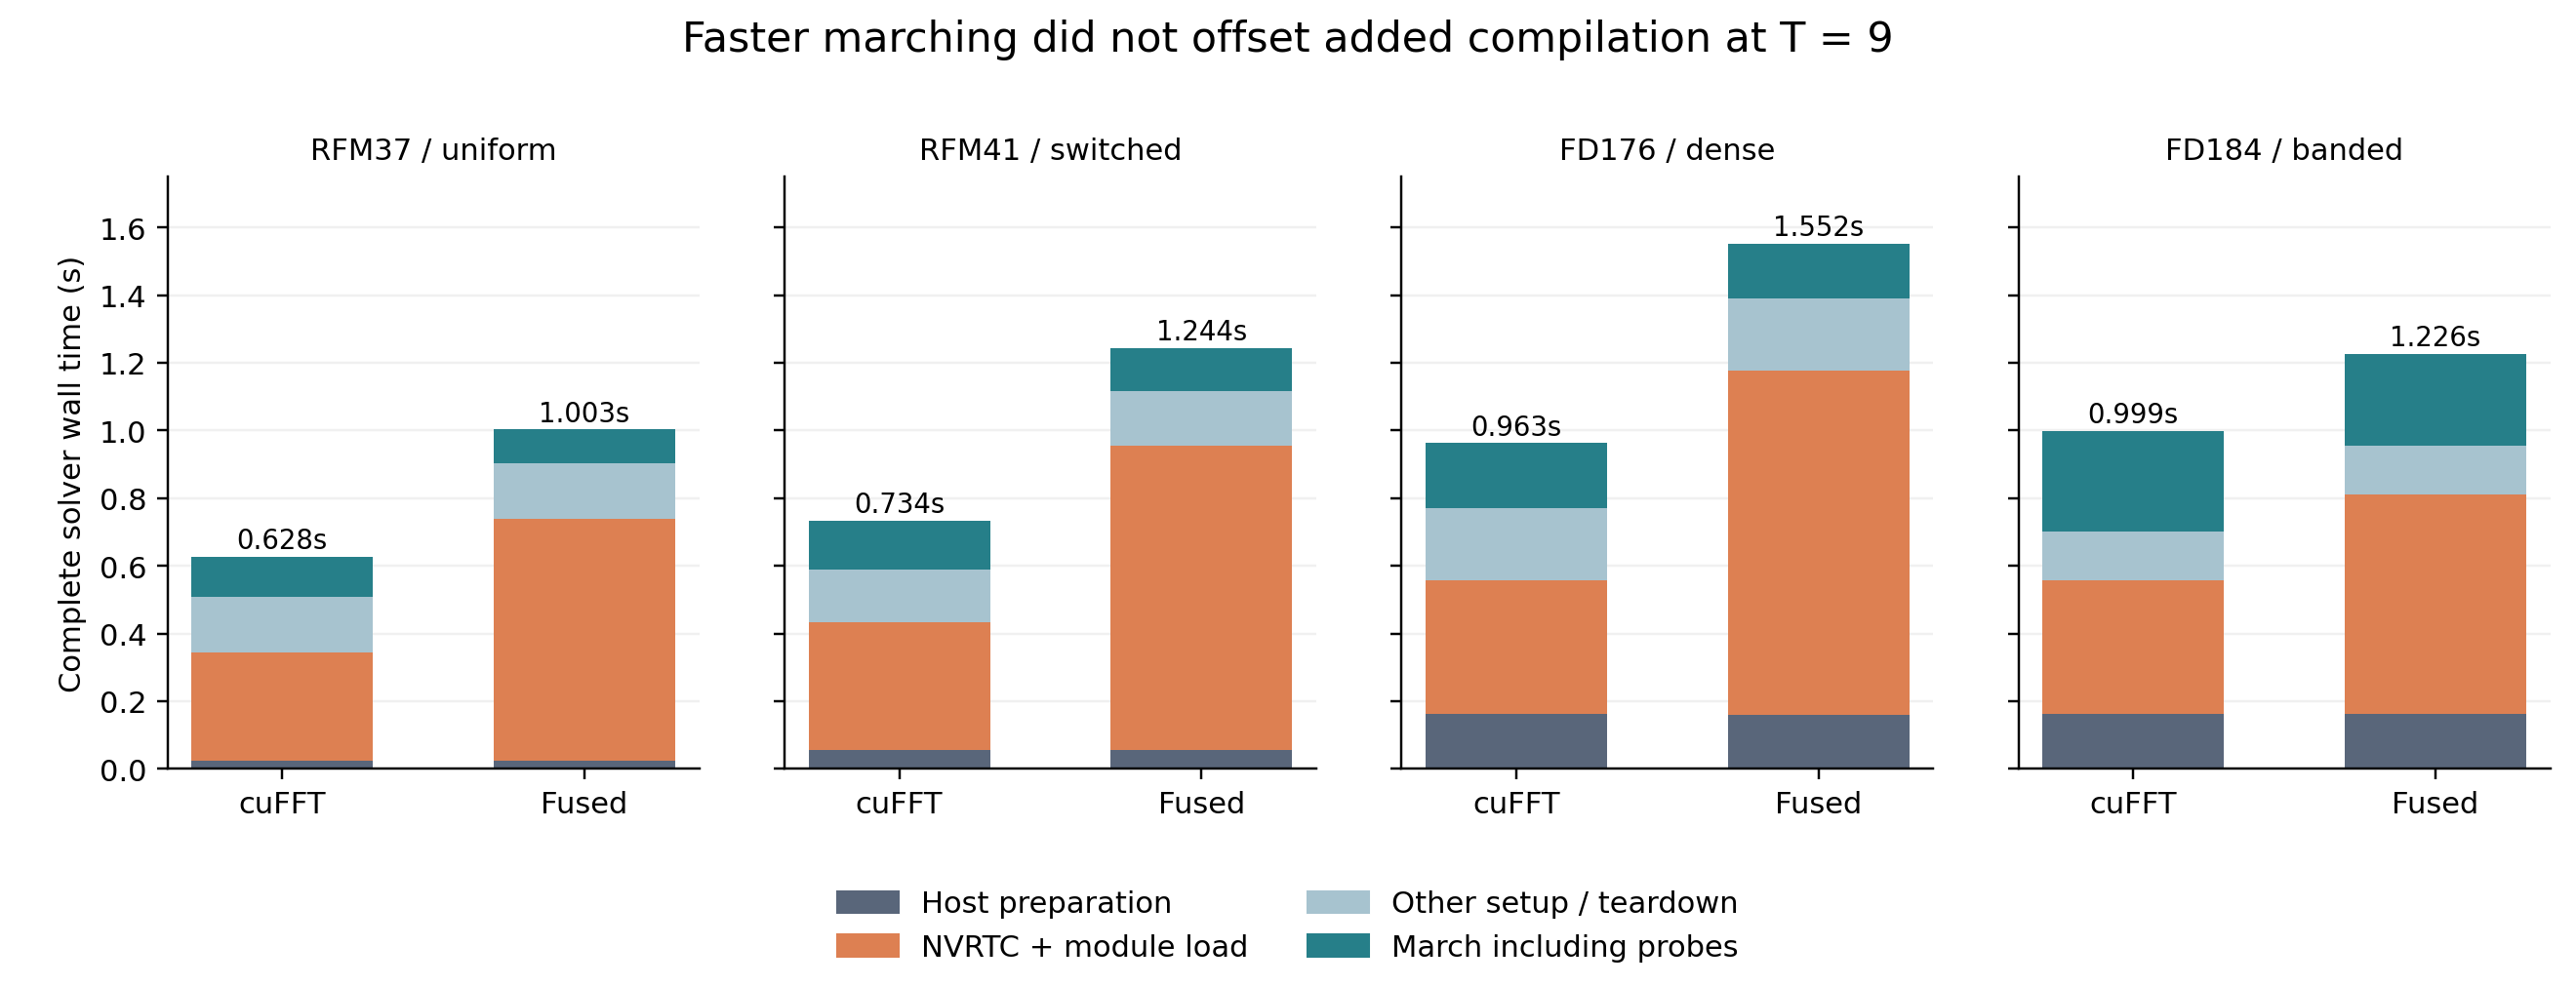
\includegraphics[width=\linewidth]{figures/t9_fusion_cost_breakdown.png}
\caption{Cost decomposition of the sequential $T=9$ fusion diagnostics. Compilation and loading are separated from the remaining runtime initialization. These diagnostic measurements identify first-use costs; they do not provide the missing final $T=72$ ranking.}
\label{fig:fusion-cost}
\end{figure}

Caching changes this tradeoff but did not remove the admission requirement. In the later strict-hit diagnostics, all four complete solver clocks improved, whereas only two of the four fresh-process comparisons improved. The candidate therefore failed its registered promotion rule and was excluded from the final $T=72$ cohort. This is an engineering selection failure, not a failure of its short-trajectory numerical tests. Extrapolating the local ratio to a long trajectory would neglect both overhead and changes in the distribution of work.

\subsection{Observation kernels and common implementation benefits}

Warp-based reduction improves a different part of the pipeline. Fixed-state probe-only nodes decrease from approximately $117$--$147\,\mu$s to $6$--$7\,\mu$s for the tested Galerkin paths, from $727.5$ to $26.2\,\mu$s for FD176, and from $760.3$ to $28.3\,\mu$s for FD184. The resulting local ratios are approximately 19--27. Five full $T=72$ checks preserve the saved states and times bitwise; the changed summation order gives a maximum relative probe difference of $9.26\times10^{-14}$. The operator does not alter the evolution equations.

Because the original FD observation node is more expensive, giving this optimization only to the proposed Galerkin solver would distort the comparison. The final cohort uses the warp observer for all relevant baselines. Multiplying hot-kernel savings by the observation count can suggest where time is spent, but it is not a substitute for the complete paired timing of the modified solver. The local ratio must not be quoted as a 19--27-fold solver speedup.

\subsection{Cache policy, startup, and amortization}

The explicit cache stores PTX compiled from project kernels; it does not store a precomputed solution, spatial matrices, CUDA context, or cuFFT plan. The key binds source, compiler options, target architecture, entry points, compiler identity, and dependency hashes. Under \texttt{strict\_hit}, a missing or corrupt artifact is an error, with no silent compilation fallback. Under \texttt{empty\_first}, each run begins with a new directory and pays for compilation, atomic writing, readback verification, and loading. Driver and operating-system caches remain in their natural state. Thus ``first use'' is an explicit policy, not a claim that the whole machine has been reset to a cold state.

Three stock PTX keys occupy 147,782 bytes. Three fresh-process installations take $2.7292$, $2.6392$, and $2.6487$~s, with a median of $2.6487$~s. Reporting only the roughly $0.93$~s NVRTC stage would omit most of this installation path. If $C$ is the complete installation cost, $H$ a subsequent hit cost, and $F$ a per-solve first-use cost under otherwise matched conditions, the amortized comparison is
\begin{equation}
\label{eq:cache-amortization}
 T_{\rm cache}(n)=C+nH,\qquad T_{\rm first}(n)=nF.
\end{equation}
A crossover requires $F>H$ and $n>C/(F-H)$. The final campaign does not provide an accepted paired estimate of $F-H$, so no measured break-even solve count is reported. The installation covers three keys; the minimum installation cost for a user needing only one key was not measured.

An earlier 50-run high-resolution campaign passed its sampled isolation check and measured median paired fresh-process speedups of 1.293 and 1.301 after import simplification for constant and piecewise RFM, while solver-time ratios stayed near unity. This identifies a startup improvement for that historical configuration. It does not replace a comparison with the stronger Legendre baseline, common warp observer, or explicit cache policies introduced later. Pooling these rows would mix different experimental treatments.

\subsection{A conditional crossover for a longer time schedule}
\label{sec:schedule-amortization}

The historical single-bridge diagnostic records about $\Delta M_0=0.119$~s of marching savings and $\Delta P=0.206$--$0.240$~s of additional preparation. These measurements come from a window marked \texttt{diagnostic\_only}, with external activity, and precede the final configuration set. They cannot supply a measured final speed ratio. They can, however, make the assumptions of a crossover estimate explicit.

Let $N$ count steps of the piecewise candidate, including the unchanged first $N_s=1024$ steps. Its $T=72$ trajectory has $N_0=8192$ steps. If the extra preparation stays constant and the saved marching time grows linearly with only the later work, the modeled candidate-minus-control time is
\begin{equation}
 \Delta T(N)=\Delta P-
       \frac{N-N_s}{N_0-N_s}\Delta M_0,\qquad
 N_* = N_s+(N_0-N_s)\frac{\Delta P}{\Delta M_0}.
 \label{eq:schedule-amortization}
\end{equation}
Substitution gives $N_*\simeq13{,}432$--$15{,}480$ candidate steps. A coarser model that scales the savings with all steps instead gives $N_*=N_0\Delta P/\Delta M_0\simeq14{,}181$--$16{,}522$. Their difference reflects the treatment of startup, not additional measurements. Thus a scale of roughly $1.5\times10^4$ steps is a conditional planning estimate, not an observed threshold. Neither model proves accuracy beyond $T=72$, constant device efficiency, or superiority to a different qualified method. Multiple short solves amortize preparation only when the relevant prepared objects are actually shared; a PTX cache alone does not share spatial matrices or FFT plans. A new longer-horizon qualification and isolated experiment are required to validate a crossover.


\section{Rejected candidates and the limits of local theory}
\label{sec:negative-results}

\subsection{Common phase coordinates and dense output layout}

The common phase-basis prototype improves local linear-algebra diagnostics but, with the existing dense device interface, increases three-phase preparation by about $37\%$--$58\%$. Table~\ref{tab:phase-setup} reports the measured values. Device storage remains $11.69$--$16.30$~MB because dense physical-coordinate operators are still generated. The prototype pays for eigendecomposition and back-transformation of wide right-hand-side blocks instead of remaining in diagonal coordinates throughout the computation.

\begin{table}[tbp]
\centering\small
\caption{Local phase-preparation measurements in milliseconds. These use the prototype's original anchor, not the later geometric-anchor rule.}
\label{tab:phase-setup}
\begin{tabularx}{\linewidth}{@{}Xrrr@{}}
\toprule
Configuration & Original & Triangular solves & Common phase basis \\
\midrule
Mid RFM & 34.27 & 47.41 & 51.96 \\
Mid Legendre & 34.81 & 44.72 & 47.73 \\
High RFM & 38.75 & 56.39 & 61.39 \\
High Legendre & 45.71 & 62.00 & 66.22 \\
\bottomrule
\end{tabularx}
\end{table}

The analytical anchor in Eq.~\eqref{eq:anchor} minimizes a condition-number upper bound. It was not timed as a new production candidate. Better transformed conditioning, fewer factorizations, less stored data, and shorter complete runtime are distinct propositions. A future implementation that keeps state in common coordinates would need corresponding reconstruction, lifting, projection, and observation operators, followed by a new floating-point and trajectory qualification. The existing prototype does not test that architecture.

\subsection{Energy structure does not guarantee coarse-step accuracy}

The Lamb--BDF2 candidate freezes an extrapolated vorticity field and solves the resulting velocity system iteratively. Appendix~\ref{sec:app-lamb} derives the discrete skew-symmetry and fixed-step energy identity, including boundary and algebraic-residual work. These properties concern the stated discrete update and norms. They do not eliminate the error introduced by extrapolating vorticity or establish accuracy at an arbitrarily large step.

At $T=16$ and step rate 128, the worst vorticity errors are $0.364950\%$ for RFM37 and $0.364784\%$ for Legendre37, satisfying the $0.5\%$ field criterion. At rate 64 they rise to approximately $161.024\%$ and $161.664\%$. The first saved failing state occurs at $t=4$, before the transverse pulse begins. At the recorded checkpoints the original-equation residuals remain at most $7.590\times10^{-10}$, and work-corrected energy defects remain at most $2.25\times10^{-15}$. A tightly solved linear system and a closed energy identity can therefore coexist with an inaccurate flow trajectory.

The qualifying rate-128 candidate requires approximately $5.03$ times as many one-dimensional FFTs as the explicit control in the same space. This count includes products needed by the iteration and residual checks; halving nominal time steps alone would hide that work. The rate-64 variants also require more transforms and fail accuracy. The branch was consequently rejected before a $T=72$ GPU comparison.

\subsection{Skipping nonlinear evaluations and changing graph schedules}

Evaluating the nonlinear term on alternate steps gives an appealing nominal reduction. Scalar tests of the corresponding history extrapolation show observed convergence orders of $1.998$--$2.016$. However, corrected Navier--Stokes pilots that activate this strategy after $t=8$ overflow near $t=9.508$ and $9.559$, while their ordinary controls complete. The failed trajectories do not supply valid accuracy or timing results. This experiment illustrates why local consistency and scalar stability probes are screening tools rather than guarantees for the driven, mode-coupled discretization.

Two implementation experiments were numerically successful but did not meet performance-selection criteria. Alternating the two existing spectral-history buffers preserves eight short paired trajectories bitwise but gives inconsistent marching changes of $-0.030$ and $+0.018$~ms in the graph-enabled pair summaries. Changing graph chunk length from 24 to 48, 64, or 128 steps preserves 36 full trajectories bitwise. Although 48 steps halves the scheduled graph launches, no alternative simultaneously meets the registered marching, solver, and fresh-process improvement criteria. These diagnostics lack full external-load isolation and do not establish small stable speed differences. The 24-step graph schedule is retained.

\section{Disposition of the final timing experiment}
\label{sec:timing-disposition}

The final design registers 160 slots across five paired blocks, two cache policies, and the qualified methods. RFM seeds are assigned by block; deterministic methods remain fixed. Both the complete solver clock and the fresh-process clock are needed for a practical result. The latter includes the declared supervisor and process-start costs. Every window must finish its prescribed sequence, satisfy numerical checks, and pass sampled isolation; failed slots are not replaced selectively with cleaner runs.

\begin{table}[tbp]
\centering\small
\caption{Final timing attempts and admissible interpretation. None provides an accepted final paired speed ranking.}
\label{tab:timing-status}
\begin{tabularx}{\linewidth}{@{}p{0.22\linewidth}XX@{}}
\toprule
Attempt & Recorded outcome & Consequence \\
\midrule
Original design & Two slots complete; the third has no confirmed timely terminal state & Incomplete paired blocks \\
First recovery & External activity in preflight; zero slots launched & Window rejected before timing \\
Final recovery & 12 attempted; 11 raw successes; terminal publication fails for the twelfth & Completion requirement fails \\
Independent load check & External CPU activity exceeds the registered budget during the final active window & Isolation fails independently \\
Numerical readback & All 12 saved trajectories match their qualification arrays; 148 slots remain unattempted & Numerical evidence retained; no ranking \\
\bottomrule
\end{tabularx}
\end{table}

In the last attempted slot, the solver writes its numerical output and exits with a successful exact-process status, but a subsequent permission error prevents publication of the terminal state. The available record does not identify the original lock holder. A later CPU-only diagnostic reproduces a file-publication failure under a controlled reader configuration, without proving that it caused the earlier event. Separately, the load monitor observes external CPU activity above $0.2$ CPU seconds per ten-second budget interval. Correcting terminal publication alone would therefore not make the recorded batch admissible.

The isolation mechanism uses sampled process identities and preflight GPU observations, not exclusive ownership enforced by the operating system. Very short processes can escape between samples, and coverage of unrelated applications is limited. Those limitations apply even to historical windows that passed the sampled check. For the final window, the recorded violations are sufficient to reject the timing regardless of the additional unobserved activity that might have existed.

No final speedup, confidence interval, or method ranking is constructed from the 11 successful raw records, from qualification durations, or by joining the two earlier slots to a later recovery. The missing high-resolution windows also prevent a claim of stable behavior across resolutions. The result is an unresolved performance ordering, rather than a measured win or loss of RFM against the strongest classical baseline.

\section{Discussion and conclusions}
\label{sec:discussion}

\subsection{What changes on a nonseparable geometry}
\label{sec:geometry-scope}

The annulus supplies more than a convenient test shape. Its metric and boundary conditions are independent of angle, so the implicit operator separates into angular blocks; the nonlinear products still couple modes. The retained radial rank $d$, number $K$ of positive modes, quadrature size $q$, and padded angular size $N$ lead to dense setup costs of order $Kd^3$ for independent modal factorizations. A step contains order $Kd^2$ modal solves, $qdK$ reconstruction and projection work, and $qN\log N$ transform work. These counts suppress fixed channel counts and the separate mean block. They describe the present implementation, not a complexity theorem for RFM in general. Differential normalization of an $n$-column raw feature matrix additionally costs order $qn^2+n^3$ in the dense regime $q\geq n$.

On an angle-dependent mapped boundary, the metric coefficients and boundary lifting generally depend on angle. Multiplication by these coefficients couples Fourier modes even in the implicit linear operator. The scalar mode equations and their separate common-phase bases then cease to be an exact factorization of the full problem. A naive dense solve with $D=O(Kd)$ coupled degrees of freedom would require $O(D^2)$ storage and $O(D^3)$ factorization. This is an avoidable dense-design cost, not a necessary lower bound: sparse local spaces, matrix-free metric products, domain decomposition, and iterative solvers are alternatives. They require a new operator design and qualification; the present GPU measurements do not test them.

The role of conditioning can be stated precisely without claiming that the annular transform removes it. Let $B$ be an SPD reference implicit operator and $A$ a mapped-domain SPD operator on the same discrete space. If the geometry and boundary construction yield constants $0<\alpha\leq\beta$ such that
\begin{equation}
 \alpha x^\top Bx\leq x^\top Ax\leq\beta x^\top Bx
 \quad\hbox{for all }x,
 \label{eq:geometry-equivalence}
\end{equation}
then the Rayleigh quotient gives
\begin{equation}
 \sigma(B^{-1/2}AB^{-1/2})\subset[\alpha,\beta],\qquad
 \kappa_2(B^{-1/2}AB^{-1/2})\leq\beta/\alpha.
 \label{eq:geometry-condition}
\end{equation}
This is a conditional preconditioning bound. We do not establish mesh-independent $\alpha,\beta$ for an arbitrary body. Distorted mappings, narrow gaps, and nonuniform local resolution can degrade them. Boundary-data approximation introduces a separate consistency error that is not controlled by this spectral bound; it need not alter the implicit matrix. Likewise, the identity $K_1=\nu I$ on the retained annular feature space is an exact-arithmetic normalization at the chosen quadrature; it does not bound every modal mass matrix, discarded approximation direction, or floating-point reconstruction error.

Local random features with partitions of unity provide a documented route to complex interfaces, including linear Stokes examples\cite{r20}. That evidence motivates an extension, but does not validate the present unsteady nonlinear solver on such geometries. A credible extension would preserve boundary and divergence constraints, compare retained dimensions and quadrature work with deterministic local spaces, and repeat both velocity/vorticity qualification and complete-cost timing. Accordingly, our compact-space and kernel conclusions are restricted to the specified separable finite annulus.

Pure radial reparameterization should be distinguished from an angle-dependent geometry. For a smooth invertible map $r=\rho(\eta)$, the metric coefficients remain independent of $\theta$. With the same angularly invariant boundary operators, Fourier orthogonality preserves the implicit modal blocks; only the radial matrices and their conditioning change. The $O(Kd^2)$ independent dense-solve cost remains applicable to the current Galerkin design. A map for an eccentric or noncircular body generally introduces angle-dependent coefficients in this representation and couples angular modes. This observation is about the chosen coordinates and operators, not a theorem that every irregular geometry requires a particular iterative algorithm.

If the coupled implicit matrix $A$ and a fixed preconditioner $B$ are SPD and the assumed spectral-equivalence inequality holds, exact-arithmetic PCG gives the standard energy-error bound\cite{r21}
\begin{equation}
 \frac{\|e_j\|_A}{\|e_0\|_A}
 \leq2\left(\frac{\sqrt{\kappa}-1}{\sqrt{\kappa}+1}\right)^j,
 \qquad \kappa=\kappa_2(B^{-1/2}AB^{-1/2})\leq\beta/\alpha.
 \label{eq:geometry-pcg-bound}
\end{equation}
For $\kappa>1$, this supplies a sufficient iteration scale $O(\sqrt{\beta/\alpha}\log(1/\varepsilon))$ for relative energy-error reduction $\varepsilon$; it is not a measured iteration count or a lower bound. The cost also includes applying $A$, solving with $B$, and reductions. The bound does not automatically apply to nonsymmetric discretizations, indefinite systems, or variable/inexact preconditioners. Smooth mapping alone has not established the needed $\alpha,\beta$ for this study. A pseudospectral metric product may use angular FFTs, whereas an assembled sparse coupling or a short Fourier convolution may use other products. Thus neither PCG nor an FFT at every matrix--vector product is mandatory, and the annular timing results cannot predict the new operator balance.



\subsection{Synthesis and conclusions}

The evidence separates numerical design from implementation. The piecewise schedule removes measured nonlinear evaluations and applies equally to RFM and Legendre. Compact qualifying spaces exist in both basis families. The custom fused operator reduces local nonlinear cost, while the warp reduction removes a substantial observation bottleneck shared by Galerkin and FD. Startup simplification and explicit caching affect different terms of the runtime. None of these facts, individually, establishes an end-to-end advantage from random features.

The closest experimentally supported bottleneck is the mismatch between a short GPU workload and its preparation costs. A historical profile assigns about $0.058$~s of a $1.70$~s full solve to host spatial preparation, approximately $3.4\%$. This is a diagnostic for that configuration, not a universal bound, but it provides little motivation for a wholesale language rewrite. Rewriting a measured hot loop can help; replacing high-level orchestration alone does not reduce the number of nonlinear evaluations, library FFTs, or device matrix operations. High-level flow solvers can already combine efficient kernels and numerical libraries~\cite{r14}.

The finite outer boundary is a major limitation. Increasing $R$ from 6 to 8 produces an unshifted maximum vorticity difference of about $50.39\%$ on the common region $r\leq4$, with accumulated phase differences included. This is a sensitivity result between finite-domain simulations, not a rigorous estimate of exact-solution error. It prevents interpreting the present $0.5\%$ qualification as an infinite-domain cylinder benchmark. The current study also does not validate pressure, drag, lift, three-dimensional turbulence, higher Reynolds numbers, or a hardware-independent speed advantage.

Advanced trained PINN methods were not measured under the same complete field, probe, and timing protocol in this phase. Consequently the paper compares a fixed-feature Galerkin discretization with its deterministic and finite-difference controls, without ranking PINN training methods. Earlier cavity and other flow studies do not automatically inherit the final annulus qualification. Broader claims require new case-specific reference and timing evidence.

The added ablation further shows that deterministic midpoint frequencies with the same analytic layers reach the field tolerance at both resolutions; randomness is not necessary for these configurations. Removing the nonzero-mode layers greatly increases error but also decreases retained rank, preventing an equal-dimensional attribution to a feature family alone. The delayed-switch controls and error profiles clarify accuracy tradeoffs without supplying a new speed ranking.

\label{sec:conclusion}
For the specified $\mathrm{Re}=100$ finite-annulus problem, all 78 registered GPU qualification trajectories meet the common velocity and vorticity criteria. The two piecewise schedules reduce nonlinear evaluations by $11.11\%$ and $9.36\%$. Fused FFT pipelines improve local and short-run marching costs but lose on first-use complete cost; the more aggressive nonlinear-update candidates fail accuracy or workload criteria. The final isolated campaign is not accepted, so a stable complete-solve speed advantage over the optimized Legendre and fourth-order spatial FD baselines remains unestablished. The defensible contribution is the explicit mathematical adaptation, kernel implementation, and evidence-based attribution of these distinct effects.

\section*{Data and code availability}

The original NS evidence corresponds to archived revision
\href{https://github.com/LStar404/rfm-navier-stokes-research/tree/6f2b3500964d3d5153b8400018236c4702ef94f8}{\texttt{6f2b350}}, retaining source, protocols, configuration identities, qualification scores, and failed attempts. Appendix~\ref{sec:app-evidence} maps these archived tables and figures to their source records. The repository is publicly accessible; the archived commit and revision inventories identify the corresponding evidence.

The new evidence is stored separately in \path{work/rfm_review_v3/}. The \texttt{ablation/} directory contains 16 CPU ablation/control trajectories, rescoring of ten frozen GPU controls, 12 capacity-construction checks, and coverage verification. The \texttt{profiles\_bridge/} directory contains four delayed-switch CPU trajectories, radial and angular error data, cellwise two-reference scores, and Parseval checks. The \texttt{maintenance/} directory contains the explicit-factory maintenance package and seven tests. Protocols, source hashes, outputs, and analysis scripts accompany the revision without overwriting the frozen evidence. These 20 new CPU trajectories do not increase the original GPU qualification count or establish a new isolated performance result. The previous standalone GPU operator example and its 36 correctness cases remain separately identified. The point-by-point response is provided as \path{response.tex} in the same manuscript project.

\FloatBarrier
\bibliography{references}
\appendix
\section{Notation, scoring grids, and reproduction order}\label{sec:app-setup}

Sections~\ref{sec:space-discretization} and \ref{sec:numerical-method} specify the model, boundary lifting, feature transformations, and weak equations. This appendix collects cross-section notation and the independent reconstruction grids. Input feature count, retained rank, quadrature size, and FFT length describe different dimensions of a solver.

\begin{table}[!htbp]
\centering\small
\caption{Principal symbols and their computational meaning.}
\begin{tabularx}{\linewidth}{@{}lX@{}}
\toprule
Symbol & Meaning \\
\midrule
$s,z,L$ & $s=\log(r/a)$, $L=\log(R/a)$, $z=s/L$ \\
$m,d,d_0$ & Input radial feature count, retained nonzero-mode rank, separate mean rank (30) \\
$K,N,q$ & Highest retained angular mode, angular FFT length, Galerkin radial quadrature count \\
$n$ & FD radial intervals; $n+1$ nodes and $n-1$ interior unknowns \\
$M_k,K_k$ & Nonzero-mode mass and viscous matrices \\
$H,h,\rho$ & Time steps before and after the bridge and ratio $h/H$ \\
$H_{\rm ref}$ & Phase whitening matrix $a_{\rm ref}M+h_{\rm ref}K$, also denoted $H$ in the analysis \\
$N_{\rm nl},C_{\rm nl}$ & True nonlinear evaluation count and effective cost per evaluation \\
\bottomrule
\end{tabularx}
\end{table}

\begin{table}[!htbp]
\centering\small
\caption{Independent physical-error reconstruction grids.}
\label{tab:app-score-grids}
\begin{tabularx}{\linewidth}{@{}Xrrr@{}}
\toprule
Grid & Radial points & Angular points & Angular shift \\
\midrule
Gauss & 123 & 433 & 0.23 \\
Uniform midpoint & 129 & 449 & 0.43 \\
Layer-refined & 144 (96/24/24) & 457 & 0.31 \\
\bottomrule
\end{tabularx}
\end{table}

The weights include $r^2\,ds\,d\theta$, and the velocity norm combines $u_r,u_\theta$. The 19 physical checkpoints are 0.5, 1, 2, 4, 6, 8, 8.125, 8.5, 9, 10, 12, 16, 24, 36, 48, 54, 60, 66, and 72. Piecewise schedules additionally save the states at $8+1/\mathrm{late\_rate}$ and $8+2/\mathrm{late\_rate}$ for implementation consistency. These are not two extra reference-scored physical checkpoints. Probe locations are $(x/D,y/D)=(1.5,0),(2.5,0),(3.5,0)$. Samples are taken at intervals of $0.125$, giving 577 times including the zero initial state. Transverse velocity and vorticity at each location give six histories.

Reproduction should first fix the archive identity, source files, and numerical references listed in Appendix~\ref{sec:app-evidence}. Check the geometry, seed, retained rank, time rates, and cache policy for each configuration. Reconstruct and score each field on every registered grid and time, then evaluate CPU/GPU implementation consistency and the piecewise triangle safeguard. Only qualified candidates proceed to independent timing; concurrent qualification elapsed times are not isolated timings. Batch completeness, terminal records, and external-load checks precede calculation of speed ratios. The revised standalone operator sample is evaluated separately: its checks cover synthetic fixed states and do not replace flow qualification.

\section{Frozen-vorticity structure and scope}
\label{sec:app-lamb}
\setcounter{equation}{0}
\renewcommand{\theequation}{B.\arabic{equation}}
\renewcommand{\theHequation}{appendix.B.\arabic{equation}}

In the real Fourier representation, the mean has weight \(1\), and the
real and imaginary parts of each nonzero mode have weight \(2\). For
frozen vorticity \(\omega^\ast\), the weak pairing is
\[
 \sum w\,\omega^\ast(u_\theta v_r-u_rv_\theta).
\]
Using the same quadrature and mutually adjoint reconstruction and
projection maps, interchanging \(u\) and \(v\) reverses the sign.
Consequently the homogeneous discrete matrix \(F\) satisfies
\(F^{\mathsf T}=-F\). This property must be checked at the discrete level.

The update with lifting, forcing, and residual work is
\begin{equation}
 \bigl[\tfrac32 M+hK-hF\bigr]x_{n+1}
 =2Mx_n-\tfrac12 Mx_{n-1}+\mathcal{L}_{n+1}+\mathcal{R}_{n+1}.
 \label{eq:lamb-step}
\end{equation}
Here \(\mathcal{L}\) contains boundary lifting and external forcing, and
\(\mathcal{R}\) is the original left-hand side minus the right-hand side
including \(\mathcal{L}\). Define
\begin{equation}
 \lVert x\rVert_M^2=x^{\mathsf T}Mx,\qquad
 G(x,y)=\lVert x\rVert_M^2+\lVert 2x-y\rVert_M^2.
 \label{eq:lamb-g}
\end{equation}
The \(K\)-weighted seminorm is defined analogously. At constant step
size \(h\), pairing \eqref{eq:lamb-step} with \(4x_{n+1}\) gives
\begin{equation}
 \begin{aligned}
 &G(x_{n+1},x_n)-G(x_n,x_{n-1})
  +\lVert x_{n+1}-2x_n+x_{n-1}\rVert_M^2
  +4h\lVert x_{n+1}\rVert_K^2\\
 &\qquad
  =4\langle x_{n+1},\mathcal{L}_{n+1}\rangle
   +4\langle x_{n+1},\mathcal{R}_{n+1}\rangle .
 \end{aligned}
 \label{eq:lamb-energy}
\end{equation}
The identity follows by expanding
\(4\langle x,\tfrac32 Mx-2My+\tfrac12 Mz\rangle\) and using skew symmetry
to cancel the \(F\) contribution. The residual \(\mathcal{R}\) is already
scaled as in \eqref{eq:lamb-step}, so its work term carries no additional
factor of \(h\). With homogeneous boundary data, zero forcing, and an
exact solve, \(\mathcal{L}=\mathcal{R}=0\) and \(G\) is nonincreasing.
Driven cases retain the right-hand side. The quantity \(G\) describes
the homogeneous velocity component. Total kinetic energy also includes
the boundary lift, and vorticity and phase errors require separate
evaluation.

Let \(A=\tfrac32 M+hK=LL^{\mathsf T}\) and \(S=L^{-1}FL^{-\mathsf T}\).
Then \(S^{\mathsf T}=-S\). In the symmetrically transformed coordinates,
\(B=I-hS\) satisfies
\[
 B^{\mathsf T}B=BB^{\mathsf T}=I-h^2S^2,\qquad
 \lVert Bz\rVert_2^2=\lVert z\rVert_2^2+h^2\lVert Sz\rVert_2^2.
\]
Hence \(\sigma_{\min}(B)\geq1\). This bound concerns the transformed
matrix. GMRES iteration count, errors from applying the coordinate
transforms, and physical accuracy require separate evaluation. The main
text reports the observed coarse-step failures and added FFT workload.

\section{Archive and verification records}
\label{sec:app-evidence}

All records below refer to commit \texttt{6f2b350}. The labels link to
the original files. Path components \texttt{v7} and \texttt{v8} identify
experimental revisions. Theoretical notes, numerical qualification,
local timing, and full-batch timing serve distinct purposes.

\begingroup
\newcommand{\ArchiveRecord}[1]{%
 \href{https://github.com/LStar404/rfm-navier-stokes-research/blob/6f2b3500964d3d5153b8400018236c4702ef94f8/#1}{\nolinkurl{#1}}}
\begin{description}
\setlength{\itemsep}{2pt}
 \item[C1 Case and boundaries]
  \ArchiveRecord{work/rfm_v6/full_case.py}
 \item[C2 Spatial spaces and matrices]
  \ArchiveRecord{work/rfm_v6/full_galerkin.py}
 \item[C3 Bridge and lifting derivation]
  \ArchiveRecord{work/rfm_v7/theory_sbdf2_single_bridge.txt}
 \item[C4 Phase pencils and scope of the anchor result]
  \ArchiveRecord{work/rfm_v8/theory_phase_pencil_scope_note.txt}
 \item[C5 Measured phase setup times]
  \ArchiveRecord{work/rfm_v8/galerkin_phase_pencil_audit_canonical_mean.json}
 \item[C6 Final 39 configurations and two-cache-policy protocol]
  \ArchiveRecord{work/rfm_v8/rank_fair_cache_qualification_output/protocol.json}
 \item[C7 Final 78 numerical qualification runs]
  \ArchiveRecord{work/rfm_v8/rank_fair_cache_qualification_output/qualification_summary.json}
 \item[C8 Rank expansion and failed candidates]
  \ArchiveRecord{work/rfm_v8/rank_parity_expansion_output/summary.json}
 \item[C9 Fused operator and short-run total cost]
  \ArchiveRecord{work/rfm_v8/fused_march_t9_output/summary.json}
 \item[C10 Isolation check for the historical startup improvement]
  \ArchiveRecord{work/rfm_v8/thin_formal_high_verification.json}
 \item[C11 Short-run Lamb accuracy and workload]
  \ArchiveRecord{work/rfm_v8/lamb_t16_qualification_output/summary.json}
 \item[C12 Disposition of the final full timing campaign]
  \ArchiveRecord{work/rfm_v8/rank_fair_cache_recovery_formal_final_closure/final_closure.json}
\end{description}
\endgroup

Table~\ref{tab:accuracy} was recomputed group by group from all 78
\texttt{independent\_score.json} files. Table~\ref{tab:workload} reads
\texttt{metadata.nonlinear\_evaluations} from \texttt{result.json} in
qualification slots \texttt{slot\_000}, \texttt{slot\_010},
\texttt{slot\_026}, and \texttt{slot\_036}.
Table~\ref{tab:fusion-events} uses fixed-state CUDA Graph event records,
and Table~\ref{tab:phase-setup} uses the local phase-setup audit.
Figures~\ref{fig:annulus-wake}, \ref{fig:wake-probes}, and
\ref{fig:fusion-cost} retain the verified plotting and data sources from
the same archive. Each performance interpretation applies within the
scope of its own timing campaign.

Source hashes are in \nolinkurl{supplement/evidence_revision.json}. The previous standalone operator and GPU checks remain in \nolinkurl{supplement/operator_sample/}; new CPU experiments and maintenance are identified in Section~\ref{sec:review-experiments} and the data-availability statement. Directory READMEs give reproduction commands.

\end{document}
